% !TeX encoding = utf8

\documentclass{beamer}

% !TeX root = latex-curto.tex
% !TeX encoding = utf8

% Personaizando o beamer
\usetheme{default}
\usecolortheme{orchid}

\usepackage[utf8]{inputenc}
\usepackage{graphicx,color}
\usepackage{amsmath,amssymb,dsfont}
\usepackage{wasysym}
\usepackage{multicol,bm}
\usepackage{etex}
\usepackage{tikz}

\setbeamersize{description width=0cm}

\frenchspacing

% logotipo do TikZ -> \Tikz
\newcommand{\Tikz}{Ti\textit{k}Z}

% emulando o pacote dingbat
%\usepackage{dingbat}
\makeatletter
\providecommand{\arkfamily}{\fontencoding{U}\fontfamily{ark}\selectfont}
\providecommand{\ark@sym}[1]{{\arkfamily\symbol{#1}}}
\newcommand{\leftthumbsup}{\ark@sym{'125}}
\newcommand{\leftthumbsdown}{\ark@sym{'104}}
\makeatother

\newcommand{\imagem}[2][]{\includegraphics[#1]{./imagens/#2}}

\newcommand{\vantagem}{{\darkgreen{\leftthumbsup}}}
\newcommand{\desvantagem}{{\red{\leftthumbsdown}}}

\newcommand{\sen}{\operatorname{sen}}

\usepackage[brazil]{babel}

\usepackage{enumerate}

%\renewcommand{\definitionname}{Definição}


\newcommand{\red}[1]{\textcolor{red}{#1}}
\newcommand{\redunder}[1]{\textcolor{red}{\underline{#1}}}
\newcommand{\green}[1]{\textcolor[rgb]{0,0.4,0}{#1}}
\newcommand{\darkgreen}[1]{\textcolor[rgb]{0,0.35,0}{#1}}
\newcommand{\blue}[1]{\textcolor{blue}{#1}}
\newcommand{\purple}[1]{\textcolor{purple}{#1}}
\newcommand{\cyan}[1]{\textcolor{cyan}{#1}}
\newcommand{\brown}[1]{\textcolor{brown}{#1}}
\newcommand{\gray}[1]{\textcolor{gray}{#1}}
\newcommand{\black}[1]{\textcolor{black}{#1}}

\theoremstyle{example}
\newtheorem*{exemplo}{Exemplo}
\newtheorem*{exemplos}{Exemplos}
\newtheorem*{dica}{Dica}


%% macros para escrever em texto puro
\newcommand{\ttbackslash}{\char92}
\let\bs\ttbackslash
\newcommand{\ttabrechaves}{\char123}
\newcommand{\ttfechachaves}{\char125}
\let\ac\ttabrechaves
\let\fc\ttfechachaves
\newcommand{\ttporcento}{\char37}
\let\pc\ttporcento
\newcommand{\ttdolar}{\char36}
\let\dolar\ttdolar
\newcommand{\ttet}{\char38}
\let\et\ttet
\newcommand{\ttcerquinha}{\char35}
\let\num\ttcerquinha
\newcommand{\ttmaior}{\char62}
\let\maior\ttmaior
\newcommand{\ttmenor}{\char60}
\let\menor\ttmenor
\newcommand{\ttaspasimples}{\char39}
\let\aspa\ttaspasimples
\newcommand{\ttgrave}{\char96}
\let\grave\ttgrave
\newcommand{\ttus}{\char95}
\let\us\ttus


\newenvironment{code}{\medskip
  \noindent\mbox{}\hspace{1cm}\begin{minipage}[t]{10cm}\ttfamily\obeylines}
  {\end{minipage}}

\newenvironment{code*}{\begin{minipage}[t]{10cm}\ttfamily\obeylines}{\end{minipage}}

\makeatletter
\renewcommand{\definition}{\@thm {\let \thm@swap \@gobble \th@definition }{theorem}{Definição}}
\makeatother

\setbeamercovered{transparent=50}

\newcommand{\vecs}[1]{(#1_1,\dots,#1_n)}
\newcommand{\vecx}[2][n]{(#2_1,\dots,#2_{#1})}

\endinput


(progn

(fset 'frame
   [?\\ ?b ?e ?g ?i ?n ?\{ ?f ?r ?a ?m ?e ?\} return ?\\ ?e ?n ?d ?\{ ?f ?r ?a ?m ?e ?\} home return up tab ?\\ ?f ?r ?a ?m ?e ?t ?i ?t ?l ?e ?\{ ?\} left])

(defun codify (prefix)
  "Substitui código puro em sua versão tipografada com as macros do
  curso de LaTeX. Com argumento prefixo, rodeia com \texttt{...}."
  (interactive "P")
  (let* ((open-curly-chackets-command "\\\\ac")
	 (close-curly-chackets-command "\\\\fc")
	 (dollar-command "\\\\dolar")
         (circ-command "\\\\textasciicircum")
	 (percent-command "\\\\pc")
         (underscore-command "\\\\us")
         (et-command "\\\\et")
         (backslash-command "\\\\bs")
	 (replace-list (list
			 (cons "\\\\" "\\\\string\\\\")
			 (cons "{" (concat open-curly-chackets-command "{}"))
			 (cons "}" (concat close-curly-chackets-command "{}"))
			 ;; fixing brackets bug
			 (cons (concat open-curly-chackets-command "{"
				       close-curly-chackets-command "{}")
			       (concat open-curly-chackets-command
                               "{}"))
                         ;; fixing bug for \\
                         (cons "\\\\string\\\\\\\\string"
                               (concat backslash-command
                                       backslash-command "{}"))
			 (cons "\\$" (concat dollar-command "{}"))
			 (cons "&" (concat et-command "{}"))
			 (cons "\\^" (concat circ-command "{}"))
                         (cons "_" (concat underscore-command "{}"))
			 (cons "%\\([^\n]*\\)\n"
			       (concat "\\\\textit{"
				       percent-command
				       "{}\\1}\n"))
			 (cons " " "\\\\ ")
			 (cons "^\\\\ \\\\ \\\\ \\\\ " "    ")
			 (cons "\n" "\\\\\\\\\n")))
	 (is-region (and transient-mark-mode
			 mark-active))
	 (beg (set-marker (make-marker) (if is-region
					    (region-beginning) (point-min))))
	 (end (set-marker (make-marker) (if is-region
					    (region-end) (point-max))))
	 (region-str-com (buffer-substring beg end))
	 (region-str-changed (copy-sequence region-str-com))
	 (deactivate-mark nil)
	 (case-repace nil)
	 (case-fold-search nil))
					; commenting
					; reclacing in string
    (dolist (rep replace-list)
      (let* ((from (car rep))
	     (to (cdr rep)))
	(setq region-str-changed
	      (replace-regexp-in-string from to region-str-changed))))
    (save-excursion
      (delete-region beg end)
      (goto-char beg)
      (cond ((equal prefix '(4)) 	; insert subs in \texttt{ }
	     (insert "\\texttt{" region-str-changed "}"))
	    ((equal prefix '(16)) ; insert commented raw + subs in \texttt{ }
	     (setq region-str-com
		   (replace-regexp-in-string "^" "%" region-str-com))
	     (insert region-str-com "\n")
	     (insert "\\texttt{" region-str-changed "}"))
	    (t		; insert only subs
	     (insert region-str-changed))))
    (set-marker beg nil)
    (set-marker end nil)))

(local-set-key (kbd "C-c C-d") 'codify)

)  ; fim do progn

%%% Local Variables: 
%%% mode: latex
%%% TeX-master: "latex-curto"
%%% End: 


\begin{document}

\title{Breve curso de \LaTeX{}}
\author[]{Prof. Miguel Frasson}
\date{ICMC}

\begin{frame}
  \titlepage
\end{frame}


% !TeX root = ../latex-curto.tex
% !TeX encoding = utf8

\part{Conceitos básicos}

\section{Começando}

\begin{frame}
  \frametitle{Como funciona o \LaTeX}

  \begin{block}{Objetivo}
    Escrever \purple{documentos}, \textit{a priori} para impressão.
  \end{block}

  %\pause

  \bigskip

  MAS pode-se fazer ...

  \begin{itemize}
  \item \green{PDF com links}, no computador
  \item \blue{Apresentações em PDF} --- como essa!
  \end{itemize}

\end{frame}

\begin{frame}

  \frametitle{Como funciona o \LaTeX}


  \begin{description}
  \item[Edição de texto] usando \purple{EDITOR} apropriado\\
    escreve-se \green{\texttt{\textit{arquivo}.tex}} que descreve o documento

\bigskip
	
    %\pause

  \item[Compilação] \purple{``roda-se''} o programa \LaTeX{} (ou equivalente)
    \begin{itemize}
    \item em geral, de dentro do editor
    \end{itemize}

\bigskip
%\pause

  \item[Visualização] é gerado arquivo 
    \green{\texttt{pdf}}  (ou outros)\\
    para \purple{visualização} ou \cyan{impressão}


  \end{description}


%   \begin{itemize}

%   \item escreve-se um arquivo \texttt{\textit{arquivo}.tex}\\
%     em que se descreve o documento na linguagem \LaTeX

%     \begin{itemize}
%     \item \blue{EDITOR} apropriado é recomendável\\ --- exemplos:
%        TeXnicCenter, Winedt, TeXmaker, etc.
%     \end{itemize}

% %\pause

%   \item roda-se o programa \LaTeX{} (ou equivalente) e ``amigos''



% %\pause

%   \item é gerado arquivo para \emph{visualização} ou \emph{impressão}\\
%     (\texttt{pdf}, \texttt{ps} ou \texttt{dvi})

%   \end{itemize}

\end{frame}


\begin{frame}
 \frametitle{Prós e contras}

  %\uncover<1>

  \begin{alertblock}{Contras...}
    \begin{itemize}\medskip
    \item Não se vê o resultado enquanto se digita\\
      (como M\$ Word)\medskip
    \item Demora-se um pouco para aprender\medskip
    \end{itemize}
  \end{alertblock}

\end{frame}

\begin{frame}
 \frametitle{Prós e contras}

   MAS (uma vez aprendido) ...



   \begin{block}{Prós... que compensam}
     \begin{itemize}\medskip

     \item \LaTeX{} é mais \green{fácil} \smiley{}\\
       (fórmulas, referências, citações, sumário, etc.)\medskip

     \item Resultado \purple{bonito} e \blue{profissional}\medskip

     \item \purple{Gratuito} e disponível para todos os sistemas\medskip

     \end{itemize}
   \end{block}

\end{frame}


\section{Instalação}

\begin{frame}
  \frametitle{Instalação}

  \begin{block}{Windows: Mik\TeX $\quad\to$ www.miktex.org}
    \show\description
    \begin{description}
    \item[\purple{Versão básica (Basic Mik\TeX\ Installer)}] \ 
      \begin{itemize}
      \item pequena ($\approx$300Mb)
      \item Precisa de internet: instala pacotes conforme são usados
      \end{itemize}
    \item[\blue{Versão completa (Mik\TeX\ Net Installer)}] \ 
      \begin{itemize}
      \item $\approx 4Gb$
      \item 1º) Download (complete) $\to$ 2º) Install
      \item Funciona sem internet
      \end{itemize}
    \item[\green{Versão Portátil (Mik\TeX\ Portable)}] \ 
      \begin{itemize}
      \item Roda direto do pendrive, não precisa instalar
      \item Precisa de internet: instala pacotes conforme são usados
      \end{itemize}

    \end{description}
  \end{block}
  
\end{frame}

\begin{frame}
  \frametitle{Instalação}

  \begin{block}{Mac: Mac\TeX}
    \begin{itemize}
    \item Versão completa e fácil de instalar
    \end{itemize}
  \end{block}
  
  \begin{block}{Linux: \TeX live}
    \begin{itemize}
    \item Oferecida entre os programas disponíveis
    \end{itemize}
  \end{block}

  \begin{block}{Online, sem instalação}
    \begin{description}
    \item[\purple{\textsc{ShareLaTeX}}]\
      \begin{itemize}
      \item \url{www.sharelatex.com}
      \item Gratuito para uso pessoal
      \end{itemize}
    \end{description}
  \end{block}


\end{frame}


\begin{frame}
  \frametitle{Editor padrão: TeXWorks}
  
  \centering
  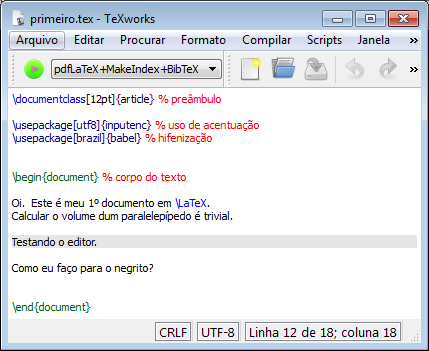
\includegraphics[scale=0.5]{./imagens/texworks-janela.png}

\end{frame}

\begin{frame}
  \frametitle{Editor padrão: TeXWorks}

  \begin{block}{TeXWorks}
    \begin{itemize}
    \item Já vem instalado quando instala-se o Mik\TeX
    \item Iterface funcional\\
      só o \blue{botão de
      rodar} 
\includegraphics[height=0.6\baselineskip]{./imagens/botao-latex.png}\ 
      e o \purple{menu de programas}\medskip

        \centerline{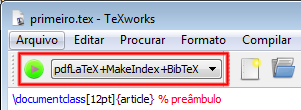
\includegraphics[scale=0.5]{./imagens/texworks-painel.png}}
      \item Visualizador de PDF com \purple{busca \LaTeX\ 
        $\leftrightarrow$ PDF}
    \end{itemize}
  \end{block}


\end{frame}




\section{A linguagem \LaTeX}

\begin{frame}

  \begin{block}{A linguagem \LaTeX}
    \begin{itemize}
      \medskip
    \item Essencialmente é \green{texto} ... \medskip %\pause
    \item ... organizado com \purple{comandos} e \blue{ambientes} \LaTeX.
      \medskip
    \end{itemize}
  \end{block}

\end{frame}

\begin{frame}
\frametitle{Básico de comandos em \LaTeX}


  \begin{block}{Comandos}

    \texttt{\purple{\bfseries{\bs}\textit{comando}}}\smallskip

    ou\smallskip

    \texttt{\purple{\bfseries{\bs}\textit{comando}}$\underbrace{\text{\red{[\textit{opcional}]}\brown{\ac\textit{arg$1$}\fc}}
        \cdots \text{\brown{\ac \textit{arg$n$}\fc}}}_{\text{parâmetros}}$}

  \end{block}

Exemplos

\begin{itemize}
\item \texttt{\purple{\string\alpha}} \quad ($\to\alpha$)
\item \texttt{\purple{\bs sqrt}\brown{\ac{}2\fc}} \quad
  ($\to\sqrt{2}$)
\item \texttt{\purple{\bs sqrt}\red{[3]}\brown{\ac{}2\fc}} \quad
  ($\to\sqrt[3]{2}$)
\end{itemize}

\end{frame}


\begin{frame}
\frametitle{Comandos em \LaTeX}

  \begin{block}{Agrupando com chaves \texttt{\ac{}...\fc{}}}

    \begin{itemize}\smallskip
    \item \purple{\texttt{Texto}} $\to$ 5 caracteres: T, e, x, t, o\smallskip
    \item \green{\texttt{\ac{}Texto\fc{}}} $\to$ 1 grupo = 1 coisa
    \end{itemize}

  \end{block}

%\pause

  \begin{exemplo}

    \begin{itemize}\smallskip
      \item  \purple{\texttt{\string\textbf}} \brown{\texttt{arg1}}\\
      $\to$ escreve \brown{\texttt{arg1}} em \textbf{negrito}\\
      \qquad \gray{(bf = bold face = negrito)}\bigskip

%\pause

    \item \blue{\texttt{\string\textbf\ Texto}} $\to$ \textbf Texto
      \quad \gray{(arg1 = T)}\smallskip
    \item \blue{\texttt{\string\textbf\ac{}Texto\fc{}}} $\to$
      \textbf{Texto} \quad \gray{(arg1 = Texto)}
      \smallskip
    \end{itemize}

  \end{exemplo}
\end{frame}



\begin{frame}
\frametitle{Ambientes}


  \begin{block}{Ambiente}\medskip

    \begin{itemize}
    \item Outro conceito importante é o \purple{ambiente}\\
      $\to$ delimita uma \green{região} do texto para um certo
      fim\medskip

%      \pause
 %   \item
      \texttt{\purple{\string\begin}\brown{\ac{}\textit{nome-do-ambiente}\fc{}}}

        \quad Texto dentro do ambiente

        \texttt{\purple{\string\end}\brown{\ac{}\textit{nome-do-ambiente}\fc{}}}
      \medskip
    \end{itemize}


  \end{block}


\medskip

%\pause

\begin{exemplos}
  
  % \begin{minipage}[t]{3cm}
  %   \begin{itemize}
  %   \item \texttt{document}
  %   \item \texttt{equation}
  %   \item \texttt{abstract}
  %   \end{itemize}
  % \end{minipage}
  % \qquad
  \begin{minipage}[t]{3cm}
    \texttt{\purple{\string\begin\brown{\ac{}equation\fc{}}}\\
        \mbox{}\ \ x\textasciicircum{}2\ -\ 1\ =\ 0\\
        \purple{\string\end}\brown{\ac{}equation\fc{}}}
  \end{minipage}
  \hfill
    \begin{minipage}[t]{6.5cm}
      \begin{equation}
        x^2-1=0       
      \end{equation}
    \end{minipage}
  \end{exemplos}

\end{frame}

\begin{frame}
 \frametitle{Estrutura básica: preâmbulo e corpo do texto}

%Exemplo de um documento simples: %(\texttt{primeiro.tex})

  \begin{code}\small
    % \documentclass[12pt]{article}     % preâmbulo
    %
    % \usepackage[latin1]{inputenc}     % uso de acentuação
    % \usepackage[brazil]{babel}        % hifenização
    %
    %
    % \begin{document}                  % corpo do texto
    %
    % Oi.  Este é meu 1º documento em \LaTeX.
    %
    % \end{document}
    \purple{\string\documentclass}\green{[12pt]\ac{}article\fc{}}\\%\ \ \ \ \ \gray{\textit{\pc{}\ preâmbulo}}a\\
\ \\
    \gray{\textit{\pc\ aqui declaram-se\ os\ pacotes\ usados,}}\ \ \
    \gray{%
      \raisebox{0cm}[0cm][0cm]{\makebox[0pt][r]{$\left.\rule{0pt}{1.1cm}\right\}$}} preâmbulo}\\
    \gray{\textit{\pc\ definem-se comandos e formatações}}\\ \ \\

%    \string\usepackage[latin1]\ac{}inputenc\fc{}a\\
%    \string\usepackage[brazil]\ac{}babel\fc{}a\\%\ \ \ \ \ \ \ \ \gray{\textit{\pc{}\ hifenização}}a\\
    \blue{\string\begin\ac{}document\fc{}}\\
\ \\
    O texto do documento vem aqui.\ \ \ \ \ \ \ \ \ \     \gray{%
      \raisebox{0cm}[0cm][0cm]{\makebox[0pt][r]{$\left.\rule{0pt}{1.1cm}\right\}$}}
      \makebox[0cm][l]{corpo do texto}}\\
\ \\
    \blue{\string\end\ac{}document\fc{}}
  \end{code}

\end{frame}


\begin{frame}
\frametitle{Classes dos documentos}

Para cada tipo, \purple{classes de documento}


\begin{block}{}\centering
  \texttt{\large\purple{\string\documentclass}\green{[$\underbrace{\text{a4paper,12pt}}_{\text{opções}}$]}\blue{\ac{}$\underbrace{\text{report}}_{\text{classe}}$\fc{}}}\par
\end{block}

\begin{block}{Classes comuns}
  \begin{itemize}
  \item \purple{\texttt{report}}, \blue{\texttt{book}}, \red{\texttt{amsbook}} $\to$ livros
  \item \blue{\texttt{article}}, \purple{\texttt{amsart}} $\to$ artigos
  \item \green{\texttt{beamer}} (como neste slide) $\to$ apresentações
  \end{itemize}
\end{block}


\end{frame}

\begin{frame}
\frametitle{Estendendo \LaTeX: pacotes}

  \begin{block}{Pacotes}
    \texttt{\purple{\string\usepackage}\green{[\textit{opções}]}\blue{\ac{}\textit{pacote}\fc{}}}
  \end{block}


\begin{block}{}
  \begin{description}
  \item[babel] hifenação e localização\qquad \gray{(opção \green{brazil})}
  \item[inputenc] acentuação\qquad \gray{(opção \green{utf8} no nosso
      caso, \green{latin1})}
%  \item[ae] boas fontes no pdf com fonte Computer Modern\qquad  \gray{(ae = almost european)}
  \item[geometry] dimensões de margens, etc.
  \item[amsmath, amssymb] %(inclua-os!) \\
    ambientes de fórmulas, símbolos ($\nexists \therefore \mathbb{R}$) etc.
  \item[graphicx] inclusão de imagens (jpg, png, pdf).
  \item[tikz] desenho de figuras
    \tikz[scale=0.15,rotate=90] \draw
    (0:1)--(2*72:1)--(4*72:1)--(6*72:1)--(8*72:1)--cycle;
    \tikz[scale=0.15] \draw (0,0) ellipse[x radius=1.7,y radius=1];
    \begin{tikzpicture}[scale=0.32]
      \draw[gray]  (72:1) arc(72:45:1) (0:1) ++(135:1) arc(135:110:1);
      \draw (0,0) -- (0:1) -- (60:1) -- cycle;      
    \end{tikzpicture}
  \item[bm] (\textbf{b}old \textbf{m}ath) fórmulas em negrito $\bm{e^{i\pi}+1 = 0}$.
  \item[multicol] Texto em várias colunas.
  \end{description}
\end{block}

\centering

  \gray{e muitíssimos outros (centenas).}

\end{frame}

%\section{Um pouco mais do básico de \LaTeX}

% \begin{frame}
% \frametitle{Caracteres especiais}

% Alguns caracteres são usados na linguagem (``reservados'')\bigskip

% \small
% \begin{tabular}{l|l|l}
%   % \purple{\texttt{\bs}} & início de comando & \blue{\texttt{\footnotesize\string\textbackslash}}  \gray{\footnotesize(\texttt{\string\\} = nova linha)} \\
%   \purple{\texttt{\dolar}} & muda modo matemático & \blue{\texttt{\string\$}} \\
%   \purple{\texttt{\et}} & tabulador & \blue{\texttt{\string\&{}}} \\
%   \purple{\texttt{\pc}} & comentário & \blue{\texttt{\string\%}} \\
%   \purple{\texttt{\num}}& def.\ comando & \blue{\texttt{\string\#}} \\
%   \purple{\texttt{\string~}} & espaço inquebrável &
%   % \blue{\texttt{\string\~\ac\fc}}\quad \gray{\footnotesize(acento til em nada)}\\
%   % \purple{\texttt{\string|}} & linhas vert. em tabelas &
%   % \blue{\texttt{\string\textbar}} \\
%   % \purple{\texttt{\string_}} & índice subescrito & \blue{\texttt{\string\_}} \\
%   % \purple{\texttt{\^{}}} & índice superscrito &
%   % \blue{\texttt{\string\^\ac\fc}} \quad \gray{\footnotesize(acento circunflexo em nada)}\\
%   % \purple{\texttt{\ac{} \fc}} & delimitador de grupos & \blue{\texttt{\string\{\
%   %    \string\}}}\\
%   %  \purple{\texttt{`` ''}} & aspas & \blue{\texttt{\grave\grave{} \aspa\aspa}}
%   %  \gray{(obs: \texttt{\aspa} $\neq$ \'{})}\\
%   %  \purple{\texttt{\maior{} \menor}} & tabulação & \blue{\texttt{\string\textgreater{} \string\textless}}
% \end{tabular}

% \end{frame}


\begin{frame}
  \frametitle{Texto e fórmulas}
  
  \begin{itemize}
  \item Digite \green{texto} normalmente.
  \item Novo parágrafo $\to$ deixe uma linha em branco.
  \item \purple{Fórmulas no parágrafo} $\to$ entre \purple{\texttt{\dolar}} e \purple{\texttt{\dolar}}: \quad
    \texttt{\purple{\dolar}\blue{\string\sqrt\ac{}x\fc{}}\purple{\dolar}}
    $\to \sqrt{x}$
  \item \blue{Fórmulas em destaque} $\to$ entre \blue{\texttt{\string\[}} e
      \blue{\texttt{\string\]}}\dots\ ou outros
  \end{itemize}

  \begin{exemplo}\small
        \texttt{Seja \purple{\dolar{}}\blue{f(x)}\purple{\dolar{}} a função dada por\\
          \purple{\string\[}\\
              \ \ \blue{f(x)\ =\ \string\frac\ac{}x\textasciicircum{}2\ +\ 1\fc{}\ac{}\string\cos\ x\fc{}}\\
              \purple{\string\]}}

        \bigskip\hrule\bigskip

        Seja $f(x)$ a função dada por
        \[
          f(x) = \frac{x^2 + 1}{\cos x}
        \]
  \end{exemplo}

\end{frame}




\begin{frame}
\frametitle{Acentos}

    \begin{block}{Escreva acentos normalmente}\medskip

      Use pacote \purple{inputenc} para acentuar normalmente\medskip

      \centering \texttt{\purple{\string\usepackage}\red{[utf8]}\blue{\ac{}inputenc\fc{}}}\medskip\par
    \end{block}

    \begin{alertblock}{Use a opção certa}
      \texttt{\purple{utf8}} -- codificação UTF-8\\
      \texttt{\purple{latin1}} -- codificação ISO 8859-1 = Latin-1      
    \end{alertblock}

  %   \begin{alertblock}{Acentos à moda antiga \hfill (não recomendado)}

  %     \begin{itemize}
  %     \item ilegível
  %     \item impede corretores ortográficos
  %     \end{itemize}

  %     \centering
  %   \begin{tabular}{p{4cm}p{2.5cm}}
  %     \green{fonte} & \green{saída} \\
  %     \blue{\texttt{\string\'orf\string\~ao}} & \'orf\~ao \\
  %     \blue{\texttt{ling\string\"ui\string\c\ac{}c\fc{}a}} & ling\"ui\c ca \\
  %     \blue{\texttt{ci\string\^encia}} & ci\^encia \\
  %   \end{tabular}
  % \end{alertblock}

\end{frame}


%%% Local Variables: 
%%% mode: latex
%%% TeX-master: "../latex-curto"
%%% End: 


%% !TeX root = ../latex-curto.tex
% !TeX encoding = utf8

\section{Pondo a mão na massa}

\begin{frame}

\frametitle{Editor padrão: \TeX works}

\imagem[height=6.5cm,keepaspectratio]{texworks-janela.png}

\end{frame}

\begin{frame}

\frametitle{Agora faça você}

Abra o programa TeXworks e digite\medskip

  \framebox{\begin{code*}\scriptsize
    % \documentclass[12pt]{article} % preâmbulo
%
    % \usepackage[utf8]{inputenc} % uso de acentuação
    % \usepackage[brazil]{babel} % hifenização
%
%
    % \begin{document} % corpo do texto
%
    % Oi.  Este é meu 1º documento em \LaTeX.
%
    % \end{document}
    \purple{\string\documentclass}\green{[12pt]}\blue{\ac{}article\fc{}}\ \ \ \ \ \gray{\textit{\pc{}\ preâmbulo}}\\
    \\
    \purple{\string\usepackage}\green{[utf8]}\blue{\ac{}inputenc\fc{}}\
    \ \ \ \ \ \ \gray{\textit{\pc{}\ uso\ de\ acentuação}}\\
    \purple{\string\usepackage}\green{[brazil]}\blue{\ac{}babel\fc{}}\ \ \ \ \ \ \ \ \gray{\textit{\pc{}\ hifenização}}\\
    \\
    \purple{\string\begin}\blue{\ac{}document\fc{}}\ \ \ \ \ \ \ \ \ \ \ \ \ \ \ \ \ \ \gray{\textit{\pc{}\ corpo\ do\ texto}}\\
      \\
      Oi.\ \ Este\ é\ meu\ 1º\ documento\ em\ \purple{\string\LaTeX}.\\
      Calcular\ o\ volume\ dum\ paralelepípedo\ é\ trivial.\\
      \\
      \purple{\string\end}\blue{\ac{}document\fc{}}
  \end{code*}}


\bigskip
Crie uma pasta\\
 e salve este arquivo nela como \green{\texttt{primeiro.tex}}.

\end{frame}

\begin{frame}
\frametitle{Rodando o \LaTeX}

  O processo é feito no TeXworks.

  \begin{itemize}
  \item Salve o arquivo \texttt{.tex}
  \item Para ``rodar o \LaTeX'', clique no botão
    \imagem[height=12pt,keepaspectratio]{botao-latex.png}\\ \imagem[height=40pt,keepaspectratio]{texworks-painel.png}
  \item Se não houveram erros, parabéns!!
  \item O visualizador PDF integrado aparecerá.

  \end{itemize}

\end{frame}

\begin{frame}
\frametitle{Compilação SEM erros}
Se compilou bem, \purple{a janela de compilaçao desaparece no final.}

\begin{center}
\imagem[width=4.5cm,keepaspectratio]{texworks-compilando.png}\ \ \ \ 
\imagem[width=4.5cm,keepaspectratio]{texworks-rodoubem.png}
\end{center}
\end{frame}

\begin{frame}
\frametitle{Compilação COM erros}
No final, a janela fica, falando a linha (aproximada) do erro.
\begin{center}
\imagem[width=8cm,keepaspectratio]{texworks-erro.png}
\end{center}
\end{frame}

\section[TeXworks]{\TeX works}

\begin{frame}
  \frametitle[Comentários mágicos no TeXworks]{Comentários mágicos no
    \TeX works}
  

  \begin{dica}{Acrescente as linhas no topo dos arquivos \texttt{.tex}}
    \begin{itemize}
    \item \purple{\texttt{\% !TEX encoding = utf8}} \\
      força o \TeX works a abrir com codificação
      certa\footnote{... no PC do seu orientador \smiley}
    \item \purple{\texttt{\% !TEX root = \textit{arquivo}}}\\
      declara arquivo raiz;\\
      compilação funciona desde qualquer arquivo
    \end{itemize}
  \end{dica}
\end{frame}

\begin{frame}
  \frametitle{Mais dicas no \TeX works}

  \begin{description}
  \item[Realce de sintaxe] Menu Formato $\to$ Realce de sintaxe $\to$
    $\bullet$~LaTeX.
  \item[aspas] Menu Formato $\to$ Aspas automáticas $\to$ $\bullet$~Unicode characters.
  \item[Preferências] Altere também estas preferências no menu Editar
    $\to$ Preferências (reinicie o editor).
  \end{description}

\end{frame}

%%% Local Variables: 
%%% mode: latex
%%% TeX-master: "../latex-curto"
%%% End: 


% !TeX root = ../latex-curto.tex
% !TeX encoding = utf8

\part{Formatação}

\begin{frame}
\frametitle{Mudando formatação}

  \begin{block}{Estilo de fontes}\small\medskip

    \begin{tabular}{l|l|p{4.5cm}}
      \green{Comando} & \green{Declaração} & \green{Efeito} \\
      \texttt{\blue{\string\textbf}\red{\ac\black{...}\fc}} & \texttt{\red{\ac}\blue{\string\bfseries}...\red{\fc}} &\rmfamily\bfseries negrito\\
      \texttt{\blue{\string\textit}\red{\ac\black{...}\fc}} & \texttt{\red{\ac}\blue{\string\itshape}...\red{\fc}} &\rmfamily\itshape itálico\\
      \texttt{\blue{\string\textsc}\red{\ac\black{...}\fc}} &
      \texttt{\red{\ac}\blue{\string\scshape}...\red{\fc}} &\rmfamily\scshape Versalete (Small Caps)\\
    \end{tabular}
  \end{block}

  \begin{block}{Tamanho das fontes}\bigskip

    \begin{tabular}{p{4cm}p{4.5cm}}
      \green{Declaração} & \green{Efeito} \\
      % \texttt{\red{\ac}\blue{\string\tiny} ...\red{\fc}} & \tiny Texto \\
      % \texttt{\red{\ac}\blue{\string\scriptsize} ...\red{\fc}} & \scriptsize Texto \\
      % \texttt{\red{\ac}\blue{\string\footnotesize} ...\red{\fc}} & \footnotesize Texto \\
      \texttt{\red{\ac}\blue{\string\small} ...\red{\fc}} & \small Texto \\
      % \texttt{\red{\ac}\blue{\string\normalsize} ...\red{\fc}} & \normalsize Texto \\
      \texttt{\red{\ac}\blue{\string\large} ...\red{\fc}} & \large Texto \\
      \texttt{\red{\ac}\blue{\string\Large} ...\red{\fc}} & \Large Texto \\
      \texttt{\red{\ac}\blue{\string\LARGE} ...\red{\fc}} & \LARGE Texto \\
      % \texttt{\red{\ac}\blue{\string\huge} ...\red{\fc}} & \huge Texto \\
      % \texttt{\red{\ac}\blue{\string\Huge} ...\red{\fc}} & \Huge Texto
    \end{tabular}
  \end{block}

\end{frame}


\begin{frame}
\frametitle{Formatação e grupos}

  \begin{itemize}
  \item Grupos (texto entre chaves)\\
    limitam o escopo de comandos de formatação.\medskip

  \item Toda formatação definida em um grupo\\
    perde o efeito ao final do grupo
  \end{itemize}\medskip
  %\pause

  \begin{exemplo}\medskip
    \begin{tabular}[c]{p{7cm}p{3cm}}
      \green{fonte} & \green{efeito} \\
      \texttt{%
        \small aaa\ \purple{\ac{}}\blue{\string\Large\string\itshape\ bbb}\purple{\fc{}}\ ccc}
                    &
                      \rmfamily
      aaa {\Large\itshape bbb} ccc
    \end{tabular}
  \end{exemplo}

\end{frame}


%%% Local Variables: 
%%% mode: latex
%%% TeX-master: "../latex-curto"
%%% End: 


% !TeX root = ../latex-curto.tex
% !TeX encoding = utf8

\section{Seções}

\begin{frame}
  \frametitle{Capítulos e seções}

  \begin{block}{Comandos de seccionamento}
    \begin{itemize}
    \item \texttt{\green{\string\chapter}\ac{}...\fc{}}
    \item \texttt{\blue{\string\section}\ac{}...\fc{}}
    \item \texttt{\blue{\string\subsection}\ac{}...\fc{}}
    \item \texttt{\blue{\string\subsubsection}\ac{}...\fc{}}
    \end{itemize}
  \end{block}

\end{frame}

\begin{frame}
  \frametitle{Seccionamento e referências}

  \begin{block}{Referenciando capítulos e seções}
    Numeração automática $\to$ use \texttt{\purple{\string\label}} e \texttt{\purple{\string\ref}}
  \end{block}

  \begin{exemplo}
    \texttt{\blue{\string\chapter}\ac{}Teoria\fc{}\ \purple{\string\label\brown{\ac{}cap:\ teoria\fc{}}}\\
      \blue{\string\section}\ac{}Notação\fc{}\ \purple{\string\label\brown{\ac{}sec:\ notacao\fc{}}}\\
      \blue{\string\section}\ac{}Resultados\fc{}\ \purple{\string\label\brown{\ac{}sec:\ resultados\fc{}}}\\
    ...\ ver\ seção\ \purple{\string\ref\brown{\ac{}sec:\ notacao\fc{}}}\ ...}

  \medskip\hrule\bigskip
  \setlength{\parindent}{0pt}
    \textbf{\large Capítulo 1 Teoria}\smallskip\par
    \textbf{1.1 Notação}\par
    \textbf{1.2 Resultados}\par
    ... ver seção 1.1 ...
  \end{exemplo}

\end{frame}

\begin{frame}
  \frametitle{Seccionamento e sumário}

  \begin{block}{Sumário}\medskip
    \blue{\texttt{\string\tableofcontents}} $\to$ sumário automático

    \begin{itemize}
    \item Comandos de seccionamento adicionam entradas ao sumário
    \end{itemize}
  \end{block}

  % \begin{dica}[``Sintonia fina'' do sumário]\medskip
  %   \texttt{\blue{\string\section}\green{[\textit{no-sumário}]}\purple{\ac{}\textit{escrito}\fc{}}}\medskip
  % \end{dica}

  \bigskip
  \begin{dica}[Incluir coisas no sumário]
    \begin{itemize}
    \item Capítulos não numerados não são incluídos no sumário
    \item \small
      \texttt{\blue{\string\chapter*}\ac{}Introdução\fc{}
        \quad\gray{\itshape\% cap. Introdução não numerado} \\
    \purple{\string\addcontentsline}\ac{}toc\fc{}\ac{}chapter\fc{}\ac{}Introdução\fc{}}
    \end{itemize}
  \end{dica}

\end{frame}

%%% Local Variables: 
%%% mode: latex
%%% TeX-master: "../latex-curto"
%%% End: 


% % !TeX root = ../latex-curto.tex
% !TeX encoding = utf8

\section{Teoremas}

\begin{frame}
  \frametitle{Teoremas, definições, etc}

  \begin{block}{Ambientes para teoremas, definições, ...}

    \begin{itemize}
    \item preâmbulo:
      \texttt{\purple{\string\usepackage}\blue{\ac{}amsthm\fc}}\medskip

    \item Tipo:

      \begin{ttfamily}\small
        \green{\string\theoremstyle}\blue{\ac{}theorem\fc{}}\ \ \ \ \gray{\textit{\footnotesize\pc{}\ titulo\ negrito,\ corpo\ itálico}}\\
        \green{\string\theoremstyle}\blue{\ac{}definition\fc{}}\ \gray{\textit{\footnotesize\pc{}\ titulo\ negrito,\ corpo\ normal}}\\
        \green{\string\theoremstyle}\blue{\ac{}remark\fc{}}\ \ \ \ \ \gray{\textit{\footnotesize\pc{}\
          titulo\ itálico,\ corpo\ normal}}
      \end{ttfamily}

    \item Declarar ambientes tipo teorema:\smallskip

      \texttt{\small\purple{\string\newtheorem}\blue{\ac{}amb\fc{}}\green{\ac{}Nome\fc{}}\brown{[contador-superior]}}
      
      ou

      \texttt{\small\purple{\string\newtheorem}\blue{\ac{}amb\fc{}}\brown{[numerar-como-amb2]}\green{\ac{}Nome\fc{}}}

    \end{itemize}
    
  \end{block}

\end{frame}

\begin{frame}
  \frametitle{Teoremas, definições, etc}

  \begin{exemplo}[no cabeçalho]
    \bigskip

    \begin{ttfamily}\small
      \green{\string\theoremstyle}\blue{\ac{}theorem\fc{}}\\
      \purple{\string\newtheorem}\blue{\ac{}teo\fc{}}\green{\ac{}Teorema\fc{}}\brown{[chapter]}\\
      \purple{\string\newtheorem}\blue{\ac{}lema\fc{}}\brown{[teo]}\green{\ac{}Lema\fc{}}\\
      \ \\
      \green{\string\theoremstyle}\blue{\ac{}definition\fc{}}\\
      \purple{\string\newtheorem}\blue{\ac{}defi\fc{}}\brown{[teo]}\green{\ac{}Definição\fc{}}\\
    \end{ttfamily}

  \end{exemplo}

  {\small Uso no próximo slide...}
  
\end{frame}

\begin{frame}
  \frametitle{Teoremas, definições, etc}

  \begin{exemplo}[no corpo do documento]
    \begin{ttfamily}\footnotesize
%      \gray{\textit{\pc{}\ já\ no\ documento\ ...}}\\
      \purple{\string\chapter}\blue{\ac{}Teoria\ dos\ números\fc{}}\\
      \ \\
      \blue{\string\begin\ac{}defi\fc{}}\brown{[Terno\ pitagórico]}\\
        \ \ Um\ \string\emph\ac{}terno\ pitagórico\fc{}\ é\ formado\ por\ três\\
        \ \ números\ naturais\ \dolar{}a\dolar{},\ \dolar{}b\dolar{}\ e\ \dolar{}c\dolar{}\ tais\ que\ \dolar{}a\textasciicircum{}2+b\textasciicircum{}2=c\textasciicircum{}2\dolar{}.\\
        \blue{\string\end\ac{}defi\fc{}}\\
      \ \\
      \blue{\string\begin\ac{}teo\fc{}}\brown{[Fermat-Wiles]}\ \purple{\string\label}\brown{\ac{}teo:\ ultimo\ teo\ fermat\fc{}}\\
        \ \ \ Não\ existe\ nenhum\ conjunto\ de\ inteiros\ positivos\\
        \ \ \ \dolar{}x\dolar{},\ \dolar{}y\dolar{},\ \dolar{}z\dolar{}\ e\ \dolar{}n\dolar{},\ com\ \dolar{}n>2\dolar{},\ tais\ que\ \dolar{}x\textasciicircum{}n+y\textasciicircum{}n=z\textasciicircum{}n\dolar{}.\\
        \blue{\string\end\ac{}teo\fc{}}\\
      \ \\
      \blue{\string\begin\ac{}proof\fc{}}\\
        \ \ Seja\ \dolar{}\string\Delta\ ABC\dolar{}\ um\ triângulo\ retângulo...\\
        \blue{\string\end\ac{}proof\fc{}}
    \end{ttfamily}

  \end{exemplo}

  {\small Resultado no próximo slide...}
  
\end{frame}

\begin{frame}
    \frametitle{Teoremas, definições, etc}

    \begin{exemplo}\medskip
      \textbf{\Large Capítulo 1 \\[2mm] Teoria dos números} \bigskip\bigskip

      \small

      \textbf{Definição 1.1 (Terno pitagórico).}  
      Um \emph{terno pitagórico} é formado por três números naturais $a$,
      $b$ e $c$ tais que $a^2+b^2=c^2$.\bigskip
      
      \textbf{Teorema 1.2 (Fermat-Wiles).} 
      \textit{Não existe nenhum conjunto de inteiros positivos $x$, $y$, $z$ e
      $n$, com $n>2$, tais que}
      \[ x^n+y^n=z^n. \]
      
      \textit{Demonstração.} 
        Seja $\Delta ABC$ um triângulo retângulo... \hfill $\square$
      

    \end{exemplo}
  
\end{frame}


%%% Local Variables: 
%%% mode: latex
%%% TeX-master: "../latex-curto"
%%% End: 


% !TeX root = ../latex-curto.tex
% !TeX encoding = utf8

\section{Dividindo}

\begin{frame}
  \frametitle{Dividindo o documento em arquivos}

  \begin{itemize}
  \item documentos grandes são divididos em capítulos e seções
  \item é mais complicado lidar com arquivos de texto muito grandes
  \item pode-se dividir o documento em partes,\\
    cada parte em arquivos separados.
  \end{itemize}

  \begin{block}{Incluir com \texttt{\string\input}}
    \medskip
    \texttt{\blue{\string\input}\purple{\ac{}arquivo\fc{}}\qquad 
      \gray{\pc\ \itshape não colocar a extensão .tex}}
    \medskip
    \begin{itemize}
    \item inclui o conteúdo do
      \purple{\texttt{\textit{arquivo}.tex}}\\
      como se este estivesse digitado ali.
    \end{itemize}
  \end{block}

\end{frame}

\begin{frame}
  \frametitle{Exemplo de dissertação típica}

  \begin{exemplo}
%    \documentclass[12pt]{report}
%    ... % preâmbulo
%    \begin{document}
%    \input{capa}
%    \input{folharosto}
%    \tableofcontents
%    \input{intro}         % cap. Introdução
%    \input{teoria}        % cap. Teoria
%    \input{aplicacoes}    % cap. Aplicações
%    \input{intro}    \ \ \ \ \ \ \ \ \ \gray{\textit{\%\ cap.\ Introdução}}
%    \input{teoria}    \ \ \ \ \ \ \ \ \gray{\textit{\%\ cap.\ Teoria}}
%    \input{aplicacoes}    \ \ \ \ \gray{\textit{\%\ cap.\ Aplicações}}
%    \bibliographystyle{acm}
%    \bibliography{teixeira}
%    \end{document}
    \texttt{\blue{\string\documentclass}[12pt]\ac{}report\fc{}\\[1mm]
      ...\ \gray{\textit{\pc{}\ preâmbulo}}\\[1mm]
      \blue{\string\begin\ac{}document\fc{}}\\[1mm]
        \ \ \ \green{\string\input}\redunder{\ac{}capa\fc{}}\\[1mm]
        \ \ \ \green{\string\input}\redunder{\ac{}folharosto\fc{}}\\[1mm]
        \ \ \ \blue{\string\tableofcontents}\\[1mm]
        \ \ \ \green{\string\input}\redunder{\ac{}intro\fc{}}
        \ \ \ \ \ \ \ \ \ \ \gray{\textit{\%\ cap.\ Introdução}}\\[1mm]
        \ \ \ \green{\string\input}\redunder{\ac{}teoria\fc{}}
        \ \ \ \ \ \ \ \ \ \gray{\textit{\%\ cap.\ Teoria}}\\[1mm]
        \ \ \ \green{\string\input}\redunder{\ac{}aplicacoes\fc{}}
        \ \ \ \ \ \gray{\textit{\%\ cap.\ Aplicações}}\\[1mm]
        \ \ \ \blue{\string\bibliographystyle}\brown{\ac{}acm\fc{}}\\[1mm]
        \ \ \ \blue{\string\bibliography}\redunder{\ac{}teixeira\fc{}}\\[1mm]
        \blue{\string\end\ac{}document\fc{}}}
  \end{exemplo}

\end{frame}


%%% Local Variables: 
%%% mode: latex
%%% TeX-master: "../latex-curto"
%%% End: 


% !TeX root = ../latex-curto.tex
% !TeX encoding = utf8

\section{Inserindo imagens}

\begin{frame}
  \frametitle{Inserindo imagens}
  
  \begin{block}{}
    \ttfamily\blue{\string\usepackage}\ac\purple{graphic\underline{x}}\fc\quad
    \gray{\textit{\pc\ no cabeçalho}}\\
    \medskip\par
    \blue{\string\includegraphics}\brown{[ajustes]}\ac{}\purple{\textit{arquivo}}\fc{}

  \end{block}

  \begin{block}{Principais ajustes}
    \begin{itemize}
    \item \brown{\texttt{scale=\textit{número}}} redimensionar a imagem
    \item \brown{\texttt{width=\textit{tamanho}}} comprimento
    \item \brown{\texttt{height=\textit{tamanho}}} altura
    \end{itemize}
  \end{block}

\end{frame}


\begin{frame}
  \frametitle{Exemplo de inserção}

   \texttt{\blue{\string\includegraphics}\brown{[width=2cm]}\purple{\ac{}smiley.pdf\fc{}}}
\qquad
      \raisebox{-0.5\height}{\imagem[width=1.5cm]{smiley.pdf}}

\bigskip

  \begin{block}{Tipos de arquivos possíveis de incluir}
    \begin{itemize}
    \item pdf
    \item jpg
    \item png
    \end{itemize}
  \end{block}

\end{frame}

\section{Figuras}

% \begin{frame}
%   \frametitle{Exemplo de tabelas}

%   \begin{exemplo}

%     \begin{columns}[c]
%       \column{6cm}
%       \texttt{\blue{\string\begin\ac{}tabular\fc{}}\redunder{\ac{}|c|r|l|\fc{}}\\
%           \ \ \green{\string\hline}\\
%           \ \ a\ \ \ \red{\et}\ bb\ \ \red{\et}\ ccc\ \purple{\bs\bs}\ \green{\string\hline}\\
%           \ \ bb\ \ \red{\et}\ ccc\ \red{\et}\ a\ \ \ \purple{\bs\bs}\ \green{\string\hline}\\
%           \ \ ccc\ \red{\et}\ a\ \ \ \red{\et}\ bb\ \ \purple{\bs\bs}\ \green{\string\hline}\\
%           \blue{\string\end\ac{}tabular\fc{}}}
%       \column{3cm}
%       \begin{tabular}{|c|r|l|}
%         \hline
%         a   & bb  & ccc \\\hline
%         bb  & ccc & a   \\\hline
%         ccc & a   & bb   \\\hline
%       \end{tabular}
%     \end{columns}

%   \end{exemplo}
% \end{frame}

\begin{frame}
  \frametitle{Figuras e tabelas}

  \begin{block}{Elementos ``flutuantes''}
    \begin{itemize}
    \item figuras ou tabelas
    \item podem ser grandes\\
      $\to$ isto dificulta seu posicionamento na página
    \item $\therefore$ figuras e tabelas podem \green{deslocar-se na
        página}\\
      $\to$ são \purple{flutuantes}
    \end{itemize}
  \end{block}

\end{frame}

\begin{frame}
  \frametitle{Figuras}

  \begin{block}{Elementos das figuras (ambiente \texttt{figure})}
    \medskip
%    \begin{figure}[posição]
%
%      (conteúdo da figura)
%
%      \caption{legenda}
%      \label{fig: label}
%    \end{figure}
    \blue{\texttt{\string\begin\ac{}figure\fc{}\brown{[lista-de-posições]}\
          \ \gray{\small\textit{\% pos:\ h,t,b,p}}}\\[2mm]
    \ \ \ \ \ }\red{\textbf{(conteúdo\ da\ figura)}}\\[2mm]
    \texttt{\ \ \purple{\string\caption\ac{}\textit{Legenda}\fc{}}\\
     \ \ \ \ \gray{\textit{\% \string\label{} SEMPRE depois do
        \string\caption{} !!}}\\
    \ \ \purple{\string\label\ac{}\textit{fig:\ label}\fc{}}\\
    \blue{\string\end\ac{}figure\fc{}}}
    \medskip
  \end{block}

\begin{block}{Posições}
  \begin{description}
  \item[h] = here = aqui
  \item[t] = top = topo da página
  \item[b] = bottom = pé da página
  \item[p] = page = em página separada
  \end{description}
\end{block}
\end{frame}

\begin{frame}
  \frametitle{Exemplo de figura (inserindo imagem)}

  \begin{exemplo}
    \medskip
    \quad
    \begin{minipage}{10cm}
    \texttt{\purple{\string\usepackage}\blue{\ac{}graphicx\fc}
      \qquad
      \gray{\pc\ no preâmbulo}}
    \bigskip
    
    \begin{ttfamily}\small
        \green{\string\begin\ac{}figure\fc{}}\red{[hb]}\\
          \mbox{}\ \ \purple{\string\centering}\\
          \mbox{}\ \ \blue{\string\includegraphics}\brown{[width=2cm]}\purple{\ac{}smiley.pdf\fc{}}\\
          \mbox{}\ \ \purple{\string\caption}\brown{\ac{}Sorria,\ você\ NÃO\ está\ sendo\ filmado.\fc{}}\\
          \mbox{}\ \ \purple{\string\label}\brown{\ac{}fig:\ sorria\fc{}}\\
          \green{\string\end\ac{}figure\fc{}}
      \end{ttfamily}
    \end{minipage}
    
    \begin{figure}[hb]
      \centering
      \imagem[width=1.5cm]{smiley.pdf}
      \caption{Sorria, você NÃO está sendo filmado.}
      \label{fig:smiley}
    \end{figure}

  \end{exemplo}

\end{frame}

%%% Local Variables: 
%%% mode: latex
%%% TeX-master: "../latex-curto"
%%% End: 


% parei

% !TeX root = ../latex-curto.tex
% !TeX encoding = utf8

\part{Modo Matemático}


\begin{frame}
  \frametitle{Estilos principais do modo matemático}
 
  \begin{block}{Estilo em linha}% ( = \texttt{\string\textstyle})
    A fórmula fica misturada ao texto na mesma linha.
  \end{block}
    \begin{exemplo}[]
      Seja $f(x) =\int_0^x \frac{\sen x}{x} dx$ a área \dots
    \end{exemplo}
    
    \medskip


  \begin{block}{Estilo em destaque}% ( = \texttt{\string\displaystyle})
    A fórmula se separa do texto, centralizada e com mais espaço.
  \end{block}
  \begin{exemplo}
    Seja
    \[
    f(x) =\int_0^x \frac{\sen x}{x} dx
    \] a área \dots
  \end{exemplo}
  


\end{frame}


\begin{frame}
  \frametitle{Modo matemático}

  \begin{block}{Estilo em linha}

    \begin{itemize}
    \item \texttt{\blue\$ ...\ \blue\$}
    \item \texttt{\blue{\string\(} ...\ \blue{\string\)}}
    \end{itemize}

  \end{block}

    \begin{exemplo}
        \texttt{A fórmula de Euler, dada por \blue{\dolar
          e\^{}\ac{}i\string\pi\fc{} + 1 = 0\dolar},\\ é considerada uma das
          mais bonitas fórmulas matemáticas.}

        \bigskip\hrule\bigskip

        A fórmula de Euler, dada por \blue{$e^{i\pi}+1=0$}, é considerada uma das
          mais bonitas fórmulas matemáticas.
    \end{exemplo}
\end{frame}

\begin{frame}
  \frametitle{Modo matemático}

  \begin{block}{Estilo destaque SEM numeração}
    \begin{itemize}
    \item \texttt{\blue{\string\[} ...\ \blue{\string\]}}
    \item \texttt{\blue{\string\begin\ac{}equation*\fc{}}\ ...\ \blue{\string\end\ac{}equation*\fc{}}}
    \end{itemize}
  \end{block}

\begin{exemplo}
  \texttt{A fórmula de Euler é dada por\\
  \blue{\string\[\\
  \mbox{}\ \ e\^{}\ac{}i\string\pi\fc{} + 1 = 0.\\
  \string\]}}

  \bigskip\hrule\bigskip

  A fórmula de Euler é dada por
  \[ \blue{e^{i\pi} + 1 = 0.}\]\smallskip
\end{exemplo}
\end{frame}

\begin{frame}
  \frametitle{Modo matemático}
  \begin{block}{Modo destaque COM numeração}
    \begin{itemize}
    \item \texttt{%\begin{equation} ... \end{equation}
        \blue{\string\begin\ac{}equation\fc{}}\ ...\ \blue{\string\end\ac{}equation\fc{}}}
%    \item equações de várias linhas
    \end{itemize}
  \end{block}

\begin{exemplo}
  \texttt{A fórmula de Euler é dada por\\
    \blue{\string\begin\ac{}equation\fc{}} \purple{\string\label\ac{}\underline{eq:\ euler}\fc{}}\\
      \mbox{}\ \  \blue{e\^{}\ac{}i\string\pi\fc{} + 1 = 0.}\\
      \blue{\string\end\ac{}equation\fc{}}\\
    ... Ver \purple{\string\eqref\ac{}\underline{eq:\ euler}\fc}.}

  \medskip\hrule\medskip

  A fórmula de Euler é dada por\blue{%
  \begin{equation} \label{eq: euler}
    e^{i\pi} + 1 = 0.
  \end{equation}}
  ... Ver \eqref{eq: euler}.
\end{exemplo}
\end{frame}


\section{Símbolos}

\begin{frame}
  \frametitle{Elementos simples}

  \begin{block}{Elementos simples}
    \begin{tabular}{lll}
      \green{Tipo} & \green{\TeX\ (modo matem.)} & \green{PDF} \\ %\hline
      Letras latinas & \blue{\tt a b x y z A B X Y} & $a b x y z A B X Y$\\
      %\hline
      Letras gregas minúsc. & \blue{\tt\string\alpha\ \string\delta} & $\alpha
      \delta$ \\ %\hline
      Letras gregas maiúsc. & \blue{\tt\string\Omega\ \string\Delta} & $\Omega
      \Delta$ \\ %\hline
      Outros símbolos & \blue{\tt\string\infty\ \string\exists}
      &$\infty\exists$\\%\hline
      & \blue{\texttt{\string\varnothing}} & $\varnothing$
    \end{tabular}
  \end{block}


\bigskip

  Mais:

  \begin{itemize}
  \item Apostila \LaTeX{} de A a B, p.\ 39.
  \item Compreensive \LaTeX\ symbols list (CTAN) \texttt{symbols-a4.pdf}
  \end{itemize}

\end{frame}

\begin{frame}
  \frametitle{Ops...}

  \begin{alertblock}{Modo matemático não é itálico!}

    \centering

    \imagem[clip,scale=0.5,bb=140 665 460 720]{diferente1.pdf}

    \medskip\hrule\medskip

    \imagem[clip,scale=0.5,bb=140 665 460 720]{diferente2.pdf}

  \end{alertblock}

\end{frame}

\begin{frame}
  \frametitle{Relações binárias}
  \begin{block}{Relações binárias}
    \centering
    \begin{tabular}{lcllcllc}
      \blue{\texttt{\string=}} & $=$ &&
      \blue{\texttt{\string\neq}} & $\neq$ &&
      \blue{\texttt{\string\approx}} & $\approx$ \\
      \blue{\texttt{\string<}} & $<$ &&
      \blue{\texttt{\string>}} & $>$ &&
      \blue{\texttt{\string\in}} & $\in$ \\
      \blue{\texttt{\string\leq}} & $\leq$ &&
      \blue{\texttt{\string\geq}} & $\geq$ &&
      \blue{\texttt{\string\not\string\in}} & $\not\in$ \\
      \blue{\texttt{\string\subset}} & $\subset$ &&
      \blue{\texttt{\string\supset}} & $\supset$ &&
      \blue{\texttt{\string\perp}} & $\perp$
    \end{tabular}
  \end{block}

  \begin{block}{Operadores binários}
    \centering
    \begin{tabular}{llllllll}
      \blue{\texttt{\string\pm}} & $\pm$ &&
      \blue{\texttt{\string\times}} & $\times$ &&
      \blue{\texttt{\string\div}} & $\div$ \\
      \blue{\texttt{\string\cap}} & $\cap$ &&
      \blue{\texttt{\string\cup}} & $\cup$ &&
      \blue{\texttt{\string\cdot}} & $\cdot$ 
    \end{tabular}
  \end{block}

\bigskip

  Mais:

  \begin{itemize}
  \item Apostila \LaTeX{} de A a B, p.\ 38.
  \item Compreensive \LaTeX\ symbols list (CTAN) \texttt{symbols-a4.pdf}
  \end{itemize}
\end{frame}


\begin{frame}
   \frametitle{Delimitadores}
  \begin{block}{Delimitadores}
    \centering
    \begin{tabular}{lcllc}
      \blue{\texttt{( )}} & $\bigl(\,\bigr)$ &&
      \blue{\texttt{[ ]}} & $\bigl[\, \bigr]$ \\[2mm]
      \blue{\texttt{\string| \string|}} & $\bigl|\,\bigr|$ &&
      \blue{\texttt{\string\| \string\|}} & $\bigl\|\, \bigr\|$ \\[2mm]
      \blue{\texttt{\string\langle\ \string\rangle}} & $\bigl\langle\,\bigr\rangle$ &&
      \blue{\texttt{\string\lbrace\ \string\rbrace}} & $\bigl\lbrace\,\bigr\rbrace$
    \end{tabular}
  \end{block}

  \def\x{\dfrac12}

  \begin{block}{Tamanhos \hfill (obs: \texttt{\string\x} = \texttt{\string\dfrac12})}
    \centering
    \begin{tabular}{lcllc}
      \blue{\texttt{(\ \black{\string\x}\ )}} & $( \x )$ &&
      \blue{\texttt{\string\left(\ \black{\string\x}\ \string\right)}} & $\left( \x \right)$  \\
      \blue{\texttt{\string\bigl(\ \black{\string\x}\ \string\bigr)}} & $\bigl( \x \bigr)$ &&
      \blue{\texttt{\string\Bigl(\ \black{\string\x}\ \string\Bigr)}} & $\Bigl( \x \Bigr)$ \\
      \blue{\texttt{\string\biggl(\ \black{\string\x}\ \string\biggr)}} & $\biggl( \x \biggr)$ &&
      \blue{\texttt{\string\Biggl(\ \black{\string\x}\ \string\Biggr)}} & $\Biggl( \x \Biggr)$
    \end{tabular}
  \end{block}
\end{frame}

\begin{frame}
  \frametitle{Fontes matemáticas}
  \begin{block}{Caligráficas}
    \texttt{\blue{\string\mathcal}\ac{}\textit{letra}\fc}
    \[
    \mathcal{A}\,\mathcal{B}\,\mathcal{C}\,\mathcal{D}\,\mathcal{E}\,\mathcal{F}\,\mathcal{G}\,\mathcal{H}\,\mathcal{I}\,\mathcal{J}\,\mathcal{K}\,\mathcal{L}\,\mathcal{M}\,\mathcal{N}\,\mathcal{O}\,\mathcal{P}\,\mathcal{Q}\,\mathcal{R}\,\mathcal{S}\,\mathcal{T}\,\mathcal{U}\,\mathcal{V}\,\mathcal{W}\,\mathcal{X}\,\mathcal{Y}\,\mathcal{Z}
    \]
  \end{block}

  \begin{block}{Blackboard Bold \hfill(\texttt{\string\usepackage\ac{}amssymb\fc{}})}
    \texttt{\blue{\string\mathbb}\ac{}\textit{letra}\fc}
    \[
    \mathbb{A}\,\mathbb{B}\,\mathbb{C}\,\mathbb{D}\,\mathbb{E}\,\mathbb{F}\,\mathbb{G}\,\mathbb{H}\,\mathbb{I}\,\mathbb{J}\,\mathbb{K}\,\mathbb{L}\,\mathbb{M}\,\mathbb{N}\,\mathbb{O}\,\mathbb{P}\,\mathbb{Q}\,\mathbb{R}\,\mathbb{S}\,\mathbb{T}\,\mathbb{U}\,\mathbb{V}\,\mathbb{W}\,\mathbb{X}\,\mathbb{Y}\,\mathbb{Z}
    \]
  \end{block}

  \begin{block}{Double Stroke \hfill(\texttt{\string\usepackage\ac{}dsfont\fc{}})}
    \texttt{\blue{\string\mathds}\ac{}\textit{letra}\fc}
    \[
    \mathds{A}\,\mathds{B}\,\mathds{C}\,\mathds{D}\,\mathds{E}\,\mathds{F}\,\mathds{G}\,\mathds{H}\,\mathds{I}\,\mathds{J}\,\mathds{K}\,\mathds{L}\,\mathds{M}\,\mathds{N}\,\mathds{O}\,\mathds{P}\,\mathds{Q}\,\mathds{R}\,\mathds{S}\,\mathds{T}\,\mathds{U}\,\mathds{V}\,\mathds{W}\,\mathds{X}\,\mathds{Y}\,\mathds{Z}
    \]
  \end{block}

\end{frame}

\section{Construções}

\begin{frame}
  \frametitle{Índices e expoentes}

  \begin{block}{Índices e expoentes}
    \centering
    \begin{tabular}{llllll}
      \blue{\texttt{x\^{}2}} & $x^2$ &&&
      \blue{\texttt{x\us n}} & $x_n$ \\
      \blue{\texttt{x\^{}2\us n}} & $x_n^2$ &&&
      \blue{\texttt{x\us\ac{}n\us k\fc}} & $x_{n_k}$ \\
      \blue{\texttt{x\us n\us k}} & \alert{erro}
    \end{tabular}
  \end{block}

  \begin{block}{Somatórios e integrais}
    \texttt{\blue{\string\sum}\green{\us\ac{}i=1\fc}\purple{\^{}\string\infty{}}
      \string\frac\ac{}1\fc{}\ac{}n\^{}2\fc{}\ =
      \string\frac\ac{}\string\pi\^{}2\fc{}\ac{}6\fc{}}
%    \vspace{-3mm}
    \[\sum_{i=1}^\infty \frac{1}{n^2} = \frac{\pi^2}{6}\]
%\vspace{-2mm}

\hrule\medskip

    \texttt{\blue{\string\int}\green{\us{}0}\purple{\^{}\string\pi}\ \string\sen\ x\string\,dx
      = 2}
    %\vspace{-3mm}
    \[\int_0^\pi \sen x\,dx=2\]
  \end{block}

\end{frame}

\begin{frame}
  \frametitle{Frações}

  \begin{block}{\texttt{\string\frac\ac{a}\fc\ac{b}\fc}}
    \begin{columns}
      \column{1cm}
      \texttt{%\frac{a}{b}
        \blue{\string\frac}\ac{}\textit{a}\fc{}\ac{}\textit{b}\fc{}}
      \column{5cm}
      \begin{tabular}{lcllc}
        Estilo em linha &&  $\frac ab$ \\[2mm]
        Estilo destaque &&  $\dfrac ab$
      \end{tabular}
    \end{columns}

  \end{block}


  \begin{block}{Forçando modo}

    \begin{itemize}
    \item \blue{\texttt{\string\tfrac}} $\to$ fração estilo em linha
      \quad\gray{\small(t $\to$ \texttt{\bs \underline{t}extstyle})}
    \item \blue{\texttt{\string\dfrac}} $\to$ fração estilo destaque
      \quad\gray{\small(d $\to$ \texttt{\bs \underline{d}isplaystyle})}
    \end{itemize}

  \end{block}

  \begin{exemplo}\centering
    \texttt{\string\[\ \string\int\ \blue{\string\frac\ac{}1\fc{}\ac{}x\fc{}}\ dx\ =\string\int\ \green{\string\tfrac\ac{}1\fc{}\ac{}x\fc{}}\ dx\ \string\]}
    \medskip\hrule
    \[ \int \blue{\frac{1}{x}} dx = \int \green{\tfrac{1}{x}} dx \]
  \end{exemplo}

\end{frame}

\begin{frame}
  \frametitle{Raízes}

  \begin{block}{Raízes}
    \centering
    \begin{tabular}{lcllc}
      \texttt{\blue{\string\sqrt}\ac{}x\fc{}} &&  $\sqrt x$ \\[2mm]
      \texttt{\blue{\string\sqrt}\red{[3]}\ac{}x\fc{}} &&  $\sqrt[3]{x}$
    \end{tabular}

  \end{block}

    \begin{exemplo}
      \texttt{%\sqrt{3-2\sqrt2} = \sqrt2-1
        \string\sqrt\ac{}3-2\string\sqrt2\fc{}\ =\ \string\sqrt2-1}
      \medskip\hrule\medskip
      \[\sqrt{3-2\sqrt2} = \sqrt2-1 \]
    \end{exemplo}

\end{frame}

\begin{frame}
  \setbeamercovered{transparent=0}

  \frametitle{Funções, limites, \dots}

  \begin{block}{Funções, limites, \dots}
    \centering
    \begin{tabular}{llllllll}
      \blue{\texttt{\string\cos}} & $\cos$ &&
      \blue{\texttt{\string\sin}} & $\sin$ &&
      \blue{\texttt{\string\tan}} & $\tan$ \\
      \blue{\texttt{\string\det}} & $\det$ &&
      \blue{\texttt{\string\log}} & $\log$ &&
      \blue{\texttt{\string\exp}} & $\exp$
    \end{tabular}
  \end{block}

  \begin{alertblock}{\texttt{\string\sen} não existe!}
    \texttt{\purple{\string\newcommand}\ac{}\blue{\string\sen}\fc{}\ac{}\green{\string\operatorname}\ac{}sen\fc{}\fc{}}
  \end{alertblock}

  \begin{exemplo}
    %\lim_{x\to 0} \frac{\sen x}{x} = 1
    \texttt{\string\lim\us\ac{}x\string\to\ 0\fc{}\
      \string\frac\ac{}\blue{\string\sen}\ x\fc{}\ac{}x\fc{}\ =\ 1}

    \medskip\hrule\medskip
    \[\lim_{x\to 0} \frac{\sen x}{x} = 1\]
  \end{exemplo}

\end{frame}

\begin{frame}
  \frametitle{Matrizes}

  \begin{exemplo}
    \begin{columns}[c]
      \column{4cm}{\ttfamily
%      \begin{pmatrix}
%         1 & 2 & 3 \\
%        -1 & 0 & 5 \\
%         0 & 3 & 4
%      \end{pmatrix}
        \blue{\string\begin\ac{}pmatrix\fc{}}\\
          \ \ \ 1\ \red{\et}\ 2\ \red{\et}\ 3\ \purple{\bs\bs}\\
          \ \ -1\ \red{\et}\ 0\ \red{\et}\ 5\ \purple{\bs\bs}\\
          \ \ \ 0\ \red{\et}\ 3\ \red{\et}\ 4\\
        \blue{\string\end\ac{}pmatrix\fc{}}}
      \column{3cm}
      \[
      \begin{pmatrix}
         1 & 2 & 3 \\
        -1 & 0 & 5 \\
         0 & 3 & 4
      \end{pmatrix}
      \]
    \end{columns}
  \end{exemplo}


  \begin{exemplo}
    {\small
    \texttt{Seja\ \dolar{}A=\brown{\string\left(}\blue{\string\begin\ac{}smallmatrix\fc{}}\\
    \ \ \ \ \ \ \ \ \ \ \ \ \ \ \ \ \ 0\ \red{\et}\ 1\ \purple{\bs\bs} -1\ \red{\et}\ 0\\
    \ \ \ \ \ \ \ \ \ \ \ \ \ \ \ \blue{\string\end\ac{}smallmatrix\fc{}}\brown{\string\right)}\dolar{}\ a\ matriz...}}

    \medskip\hrule\medskip

    Seja \blue{$A=\left(\begin{smallmatrix}
        0 & 1 \\ -1 & 0
      \end{smallmatrix}\right)$} a matriz...    
  \end{exemplo}

\end{frame}

\section{Fórmulas de várias linhas}

%\setcounter{equation}{0}

\begin{frame}
  \frametitle{Ambientes de várias linhas}


  \begin{block}{Alinhado}
      \texttt{%
%       \begin{align}
%         a_1 & = b_1 + c_1 \label{eq1}\\
%         a_2 & = b_2 + c_2
%                -d_2 + e_2 \nonumber
%       \end{align}
    \ \ \ \blue{\string\begin\ac{}align\fc{}}\\
    \ \ \ \ \ a\us{}1\ \red{\et}{}\ =\ b\us{}1\ +\ c\us{}1\
    \purple{\string\label\brown{\ac{}eq:\ align\fc{}}}\ \red{\bs\bs}{}\\
    \ \ \ \ \ a\us{}2\ \red{\et}{}\ =\ b\us{}2\ +\ c\us{}2\\
    \ \ \ \ \ \ \ \ \ \ \ \ -d\us{}2\ +\ e\us{}2\ \green{\string\nonumber}\\
    \ \ \ \blue{\string\end\ac{}align\fc{}}\\
    \ \ \ Segue da equação \purple{\string\eqref{\brown{\ac{}eq:\
          align\fc}}} ...}

\medskip\hrule

      \begin{align}
        a_1 &= b_1 + c_1 \label{eq: align} \\
        a_2 &= b_2 + c_2
              -d_2 + e_2 \nonumber
      \end{align}
      Segue da equação \eqref{eq: align} \dots
  \end{block}
\end{frame}

\begin{frame}
  \frametitle{Ambientes de várias linhas}
  \begin{block}{Centralizado}
      \texttt{%
%       \begin{gather}
%         a_1 & = b_1 + c_1 \label{eq1}\\
%         a_2 & = b_2 + c_2
%                -d_2 + e_2 \nonumber
%       \end{gather}
    \ \ \ \blue{\string\begin\ac{}gather\fc{}}\\
    \ \ \ \ \ a\us{}1\ =\ b\us{}1\ +\ c\us{}1\
    \purple{\string\label\brown{\ac{}eq:\ gather\fc{}}}\ \red{\bs\bs}{}\\
    \ \ \ \ \ a\us{}2\ =\ b\us{}2\ +\ c\us{}2\\
    \ \ \ \ \ \ \ \ \ \ -d\us{}2\ +\ e\us{}2\ \green{\string\nonumber}\\
    \ \ \ \blue{\string\end\ac{}gather\fc{}}\\
    \ \ \ Segue da equação \purple{\string\eqref{\brown{\ac{}eq:\
          gather\fc}}} ...}

\medskip\hrule

      \begin{gather}
        a_1 = b_1 + c_1 \label{eq: gather} \\
        a_2 = b_2 + c_2
              -d_2 + e_2 \nonumber
      \end{gather}
      Segue da equação \eqref{eq: gather} \dots
  \end{block}
\end{frame}

\begin{frame}
  \frametitle{Numeração e referência}

  \begin{block}{Numero ou não?}
    \centering
    \begin{tabular}{lll}
      \green{COM numeração} && \green{SEM numeração}\\ %\hline
      \blue{\texttt{equation}} && \blue{\texttt{equation\purple{*}}} \\
      \blue{\texttt{align}} && \blue{\texttt{align\purple{*}}} \\
      \blue{\texttt{gather}} && \blue{\texttt{gather\purple{*}}}
    \end{tabular}
  \end{block}

\end{frame}


%%% Local Variables: 
%%% mode: latex
%%% TeX-master: "../latex-curto"
%%% End: 



% % !TeX root = ../latex-curto.tex
% !TeX encoding = utf8

\section{Listas}

\begin{frame}
  \frametitle{Listas}
  \begin{block}{Tipos de listas}
    \begin{itemize}
    \item não numeradas
    \item numeradas
    \item descritivas
    \item podem ser ``encaixadas'' (ou ``aninhadas'')
    \end{itemize}
  \end{block}

\end{frame}

\begin{frame}
  \frametitle{Listas não numeradas}
  \begin{block}{Listas não numeradas: ambiente \texttt{itemize}}
    \texttt{\blue{\string\begin\ac{}itemize\fc{}}\\
        \purple{\string\item}\ ...\\
        \purple{\string\item}\ ...\\
        \blue{\string\end\ac{}itemize\fc{}}}
  \end{block}

  %\pause

  \begin{exemplo}

    \begin{columns}[c]
      \column{4cm}
      \texttt{\blue{\string\begin\ac{}itemize\fc{}}\\
          \purple{\string\item}\ aaa\\
          \purple{\string\item}\ bbb\\
          \purple{\string\item}\ ccc\\
          \blue{\string\end\ac{}itemize\fc{}}}
      \column{3cm}
      \begin{itemize}
      \item aaa
      \item bbb
      \item ccc
      \end{itemize}
    \end{columns}

  \end{exemplo}


\end{frame}


\begin{frame}
  \frametitle{Listas numeradas}
    \begin{block}{Listas numeradas: ambiente \texttt{enumerate}}
    \texttt{\blue{\string\begin\ac{}enumerate\fc{}}\\
        \purple{\string\item}\ ...\\
        \purple{\string\item}\ ...\\
        \blue{\string\end\ac{}enumerate\fc{}}}
  \end{block}

  %\pause
    \begin{exemplo}

    \begin{columns}[c]
      \column{4cm}
      \texttt{\blue{\string\begin\ac{}enumerate\fc{}}\\
          \purple{\string\item}\ aaa\\
          \purple{\string\item}\ bbb\\
          \purple{\string\item}\ ccc\\
          \blue{\string\end\ac{}enumerate\fc{}}}
      \column{3cm}
      \begin{enumerate}
      \item aaa
      \item bbb
      \item ccc
      \end{enumerate}
    \end{columns}

  \end{exemplo}


\end{frame}



\begin{frame}
  \frametitle{Exemplo com listas aninhadas}

  \begin{exemplo}[com listas aninhadas]

    \begin{columns}[c]
      \column{4cm}
      \texttt{\blue{\string\begin\ac{}enumerate\fc{}}\\
          \purple{\string\item}\ aaa\\
          \purple{\string\item}\ bbb\\
          \ \ \green{\string\begin\ac{}itemize\fc{}}\\
            \ \ \purple{\string\item}\ ccc\\
            \ \ \purple{\string\item}\ ddd\\
            \ \ \green{\string\end\ac{}itemize\fc{}}\\
          \purple{\string\item}\ eee\\
          \blue{\string\end\ac{}enumerate\fc{}}}
      \column{3cm}
      \begin{enumerate}
      \item aaa
      \item bbb
        \begin{itemize}
        \item ccc
        \item ddd
        \end{itemize}
      \item eee
      \end{enumerate}
    \end{columns}

  \end{exemplo}

\end{frame}

\begin{frame}
  \frametitle{Lista descritiva}
    \begin{block}{Listas descritivas: ambiente \texttt{description}}
    \texttt{\blue{\string\begin\ac{}description\fc{}}\\
        \purple{\string\item}\redunder{[\textit{nome1}]}\ ...\\
        \purple{\string\item}\redunder{[\textit{nome2}]}\ ...\\
        \blue{\string\end\ac{}description\fc{}}}
  \end{block}

%\pause
  \begin{exemplo}

    \begin{columns}[c]
      \column{5.5cm}
      \texttt{\blue{\string\begin\ac{}description\fc{}}\\
          \purple{\string\item}\redunder{[aaa]}\\
          \ \ \ é\ sequência\ de\ três\ a's\\
          \purple{\string\item}\redunder{[bbb]}\\
          \ \ \ é\ sequência\ de\ três\ a's\\
          \purple{\string\item}\redunder{[ccc]}\\
          \ \ \ é\ sequência\ de\ três\ a's\\
          \blue{\string\end\ac{}description\fc{}}}
      \column{4.2cm}
      \begin{description}
      \item[aaa] é sequência de três a's
      \item[bbb] é sequência de três b's
      \item[ccc] é sequência de três c's
      \end{description}
    \end{columns}

  \end{exemplo}

\end{frame}


%%% Local Variables: 
%%% mode: latex
%%% TeX-master: "../latex-curto"
%%% End: 


% % !TeX root = ../latex-curto.tex
% !TeX encoding = utf8

\section{Bibliografia}

\begin{frame}
  \frametitle{Bibliografia}

  \begin{block}{Jeitos de implementar a bibliografia}
    \begin{itemize}
    \item \vantagem\ automático
    \item \desvantagem\ manual

    \end{itemize}

  \end{block}
\end{frame}

\begin{frame}
  \frametitle{Bibliografia manual}

  \begin{block}{Usando bibliografia manual \leftthumbsdown}
    \begin{itemize}
    \item Formata-se as entradas manualmente\\
      usando o ambiente \blue{\texttt{thebibliography}}\\
      em que cada entrada começa com
      \texttt{\green{\string\bibitem}\purple{\ac{}\textit{label}\fc{}}}\medskip
    \item \texttt{\blue{\string\cite}\purple{\ac{}label\fc{}}} no
      texto para citar
    \end{itemize}
  \end{block}

  \begin{alertblock}{Cuidado}
    Formatação manual é suscetível a inconsistências.
  \end{alertblock}
\end{frame}

\begin{frame}
  \frametitle{Bibliografia automática}

  \begin{block}{Usando Bib\TeX\ \leftthumbsup}
    \begin{itemize}
    \item Mantém-se um arquivo pessoal com extensão
      \blue{\texttt{.bib}}\\
      Ex: \purple{\texttt{teixeira.bib}}
    \item No arquivo \texttt{.bib}, cada entrada tem um \purple{\texttt{label}}.
    \item No final do documento, inclui-se as linhas
      \begin{quote}\upshape
        \ttfamily
        \blue{\string\bibliographystyle}\brown{\ac{}$\overbrace{\text{acm}}^{\text{estilo}}$\fc{}}\\[2mm]
        \blue{\string\bibliography}\redunder{\ac{}teixeira\fc{}}
      \end{quote}
    \item \texttt{\blue{\string\cite}\purple{\ac{}label\fc{}}} no
      texto para citar
    \end{itemize}
  \end{block}

\end{frame}

\begin{frame}
  \frametitle{Entradas no arquivo \texttt{.bib}}

  \begin{exemplo}
    A maioria das obras e artigos tem a entrada Bib\TeX{} pronta.

    \begin{itemize}
    \item No \blue{MathSciNet (\url{www.ams.org/mathscinet})},\\
      procurar obra
    \item Na página da obra, tem uma caixa de combo\\
      \ \ \ \ \ \ {\textit{Select alternative format}}
    \item Escolha \textbf{Bib\TeX}
    \item Mude o label à escolha
      e inclua no \texttt{.bib}
    \end{itemize}
  \end{exemplo}
\end{frame}

%%% Local Variables: 
%%% mode: latex
%%% TeX-master: "../latex-curto"
%%% End: 



% % !TeX root = ../latex-curto.tex
% !TeX encoding = utf8

\section{TikZ}

\begin{frame}
  \frametitle{\Tikz}
  
  \begin{itemize}
  \item O \Tikz\ é uma linguagem que gera figuras, a partir de uma
    descrição da mesma em termos de linhas, formas e texto.
  \item gráficos são vetoriais e de alta qualidade
  \item já são parte do documento \tikz \draw[color=blue,thick] (0,0)
    circle (.7ex); sendo \tikz \draw[rotate=20,purple,thick] (0,0) rectangle
    (1ex,.6ex); fáceis 
    \tikz \draw[thick,green!50!black] (0,0) -- (1ex,0) -- (60:1ex) --cycle;
    de misturar.
  \end{itemize}


 
\end{frame}

\begin{frame}
  \frametitle{Figuras com \Tikz}

  \begin{itemize}
  \item Usar pacote \green{\texttt{tikz}} no preâmbulo
  \item Usar ambiente \blue{\texttt{tikzpicture}}
  \item Dentro do ambiente, usar \brown{comandos} como\\
    \purple{\texttt{\bs draw}} --- para traçar linhas\\
    \purple{\texttt{\bs fill}} --- para áreas preenchidas\\
    \purple{\texttt{\bs node}} --- para escrever texto\\
    que \green{terminam com ponto-e-vírgula ``\texttt{;}''}
  \item tem \green{parâmetros opcionais} para alterar estilos
    de linha e preenchimento

  \end{itemize}
\end{frame}

\begin{frame}
  \frametitle{Exemplo}

\begin{multicols}{2}
\begin{code*}\footnotesize
\string\begin\ac{}tikzpicture\fc{}\\
\string\draw[blue]\ (0,1)\ --\ (1,0);\\
\string\end\ac{}tikzpicture\fc{}
\end{code*}

\begin{tikzpicture}
\draw[->,blue]  (0,1) -- (1,0);
\end{tikzpicture}
\end{multicols}
  
\end{frame}

\section{Coordenadas e marcas aos pontos}

\begin{frame}
  \frametitle{Pontos}

  \begin{block}{Pontos}
    Dois valores entre parênteses.
  \end{block}
\bigskip

  Podem ser em \green{coordenadas}
  \begin{description}
  \item[cartesianas] valores $(x,y)$ separados por \green{vírgula ``\texttt{,}''} --- \texttt{(0,1)}
  \item[polares] valores $(\theta:r)$ separados por \green{2-pontos
    ``\texttt{:}''} --- \texttt{(30:1)}
  \end{description}
\end{frame}

\begin{frame}
  \frametitle{Coordenadas em valor absoluto ou relativo}

  \begin{block}{Tipos de coordanadas}
    \begin{description}
    \item[absoluto] Determina o ponto\\
      \blue{\texttt{(1,0)}} --- ponto de coordenadas $(1,0)$.
    \item[relativo] Adiciona à posição atual: comece ponto com
      \green{\texttt{++}}
      \blue{\texttt{++(1,0)}} --- se o ponto anterior era $(2,2)$, vai
      para o ponto $(3,2)$.
    
    \item[cruzamento] Ponto definido pelo cruzamento da \blue{vertical horizontal por um ponto A} e pela \green{horizontal por outro ponto B}:\\
      \texttt{\green{(}{\blue{\textit{A}} \purple{|-} \blue{\textit{B}}\green{)}}}
    % \item[relativo sem atualização] Adiciona à posição atual\\
    %   mas \red{não atualiza posição}:\\ comece ponto com \green{\texttt{+}}.

    %   Exemplo: \blue{\texttt{+(1,0)}} --- se o ponto anterior era
    %   $(2,2)$, denota o ponto $(3,2)$, mas ponto atual fica em
    %   $(2,2)$.
    \end{description}
  \end{block}

\end{frame}

\begin{frame}

  \frametitle{Exemplo}

\centering

  \begin{tikzpicture}[scale=4,>=stealth]
    \draw[gray,dotted] (50:1) coordinate (A) -- node[midway,above left] {$1$}
    (0,0) coordinate (O) -- (1.5,0);
    \draw[thin,->,gray] (0:.2) arc (0:50:.2);
    \node[gray] at (20:.3) {$50^{\circ}$};
    \fill (0,0) circle (.3pt) (A) circle (.3pt)
          ++(-30:.5) coordinate (B) circle (.3pt)
          (O |- A) coordinate (OA) circle (.3pt);

    \draw[gray,dotted] (A) +(.3,0) -- +(-1.3,0) (0,-.2)--(0,.9); 
    \draw[gray,dotted] (A) -- node[midway,below left=-1mm] {\scriptsize$0.5$} (B) ;
    \begin{scope}[shift={(A)}]\scriptsize
      \draw[thin,->,gray] (0:.2) arc (0:-30:.2);
      \node[gray] at (-12:.3) {$-30^{\circ}$};
      
    \end{scope}


    \node[left] at (O) {\blue{\texttt{(0,0)}}};
    \node[above] at (A) {\green{\texttt{(50:1)}}};
    \node[above left] at (OA) {\purple{\texttt{(0,0 |- 50:1)}}};
    \node[right] at (B) {\red{\texttt{(50:1) ++(-30:.5)}}};
  \end{tikzpicture}
\end{frame}


\begin{frame}
  \frametitle{Comando \texttt{coordinate}}

  \begin{block}{\texttt{coordinate}}
  Após escrever um ponto, adicionar\\
    \mbox{}\hfill\purple{\texttt{coordinate (\texttt{nome})}}\hfill\mbox{} \\
    para nomeá-lo para usar em comandos futuros.
  \end{block}

  \begin{exampleblock}{}\small
    \texttt{\string\begin\ac{}tikzpicture\fc{}\\
    \ \ \string\draw[->]\ \purple{(0,0)\ coordinate\ (A)}\ --
    \blue{(30:1)\ coordinate\ (B)};\\
    \ \ \string\draw[thick,\ dotted]\ \purple{(A)}\ --\ (1,0)\ --\ \blue{(B)};\\
    \string\end\ac{}tikzpicture\fc{}\\}

\centering
    \begin{tikzpicture}[scale=2]
      \draw[->] (0,0) coordinate (A) -- (30:1) coordinate (B);
      \draw[thick, dotted] (A) -- (1,0) -- (B);
    \end{tikzpicture}

  \end{exampleblock}

\end{frame}

\section{Caminhos}

\begin{frame}
  \frametitle{Tipos de caminhos}

  \begin{block}{Tipos de caminhos}
    \begin{itemize}
    \item segmentos
    \item círculos
    \item arcos de circunferência
    \item linhas especificando ângulos de saída e chegada
    \item béziers
    \item parábolas
    \item gráficos de funções
    \end{itemize}
  \end{block}

\medskip

\begin{block}
  {Caminhos podem ser}
  \begin{itemize}
  \item abertos
  \item fechados (termina com \texttt{-{}- cycle})
  \end{itemize}
\end{block}
\end{frame}


\begin{frame}
  \frametitle{Segmentos}

  \begin{block}{Segmentos}
    Sequência de pontos ligados por \texttt{--}.
  \end{block}

\begin{exampleblock}{}\small
\begin{code*}
\string\begin\ac{}tikzpicture\fc{}\\
\ \ \string\draw\ (90:1) -- (90+120:1) -- (90-120:1) -- cycle;\\
\string\end\ac{}tikzpicture\fc{}
\end{code*}
\medskip

\centering
\begin{tikzpicture}
\draw (90:1) -- (90+120:1) -- (90-120:1) -- cycle;
\end{tikzpicture}
\end{exampleblock}

\end{frame}





\begin{frame}
\frametitle{Retângulos}

\begin{block}{Retângulo}\ttfamily
\purple{\string\draw} ... \texttt{\green{\textit{ponto-inicial}} \blue{rectangle} \green{\textit{ponto-final}};}
\end{block}

\bigskip 

\begin{code*}
\string\draw\ \green{(0,0)} \blue{rectangle} \green{(2,1)}  \blue{rectangle} \green{(3,3)};

\bigskip\centering

\tikz{\draw (0,0) rectangle (2,1) rectangle (3,3);} 
\end{code*}

\end{frame}









\begin{frame}
  \frametitle{Círculos}

  \begin{block}{Círculos (centro no ponto atual)}\ttfamily
    \purple{\string\draw} ... \blue{\textit{ponto-centro}} \green{\texttt{circle (\textit{raio})};}
  \end{block}

\bigskip

\begin{multicols}{2}

\begin{code*}\footnotesize
\string\begin\ac{}tikzpicture\fc{}\\
\mbox{}\ \ \string\draw[thick]\ (0,0) \purple{circle\ (1)};\\
\mbox{}\ \ \string\draw\ (0,0)\ --\\
\mbox{}\ \ \ \ \ \gray{\textit{\pc{} escrevendo no meio do segmento}}\\
\mbox{}\ \ \ \ \ \green{node[right]\ \ac{}\dolar{}r=1\dolar{}\fc{}}\\
\mbox{}\ \ \ \ (0,1);\\
\string\end\ac{}tikzpicture\fc{}
\end{code*}

\mbox{}\hfill\begin{tikzpicture}[scale=1.5]
  \draw[thick] (0,0) circle (1);
  \draw (0,0) -- node[pos=.5,right] {$r=1$} (0,1);
\end{tikzpicture}

\end{multicols}

% \bigskip

% \begin{multicols}{2}

% \begin{code*}\scriptsize
% \string\begin\ac{}tikzpicture\fc{}\\
% \string\draw[thick]\ +(1,0)\ --\ +(0,1)\ --\ +(-1,0)\ --\ +(0,-1)\ --\ cycle;\\
% \string\fill\ circle\ (.1);\\
% \string\end\ac{}tikzpicture\fc{}
% \end{code*}

% \ \\\hfill \begin{tikzpicture}[scale=.5]
% \draw[thick] +(1,0) -- +(0,1) -- +(-1,0) -- +(0,-1) -- cycle;
% \fill circle (.1);
% \end{tikzpicture}


%\end{multicols}


\end{frame}

\begin{frame}
  \frametitle{Arcos de circunferência}
  \begin{block}{Arcos}
    \texttt{\purple{\string\draw} ... \red{\textit{ponto-inicial}}\\
      \mbox{}\ \ \ \ \ \ \blue{arc} (\green{\textit{ângulo-inicial}}:\blue{\textit{ângulo-final}}:\purple{\textit{raio}})}\bigskip

    O arco \blue{inicia no ponto atual.}\medskip

    Isto é ideal para colar
    vários arcos para uma curva suave.
  \end{block}

\bigskip

  \begin{alertblock}{Parece antinatural}
    \red{O ponto atual não é o centro}, como costuma-se pensar no início.
  \end{alertblock}

\end{frame}

\begin{frame}
  \frametitle{Exemplo com \texttt{arc}}

  \begin{exampleblock}{Ângulos opostos pelo vértice}
    \medskip

%    \begin{minipage}{.9\linewidth}
\scriptsize\ttfamily
    \purple{\string\begin\ac{}tikzpicture\fc}\\
    \mbox{}\ \ \string\draw\ (-1,0)\ --\ (2,0);\ \ \ \ \ \ \ \ \ \ \ \ \ \ \ \ \ \ \ \gray{\textit{\pc{}\ reta\ inferior}}\\
    \mbox{}\ \ \string\draw\ (-1,0\ |-\ 50:1)\ --\ (2,0\ |-\ 50:1);\ \ \ \gray{\textit{\pc{}\ paralela\ superior}}\\
    \mbox{}\ \ \string\draw\ (50:-.7)\ --\ (50:1.7);\ \ \ \ \ \ \ \ \ \ \ \ \ \ \gray{\textit{\pc{}\ transversal}}\\
    \mbox{}\ \ \string\draw\ (0:.3)\ \blue{arc\ (0:50:.3)};\ \ \ \ \ \ \ \ \ \ \ \ \ \ \gray{\textit{\pc{}\ arco\ inferior}}\\
    \mbox{}\ \ \string\draw\ (25:.25)\ --\ (25:.35);\ \ \ \ \ \ \ \ \ \ \ \ \ \ \gray{\textit{\pc{}\ marquinha\ inferior}}\\
    \mbox{}\ \ \gray{\textit{\pc{}\ usando\ coordenadas\ relativas\ agora}}\\
    \mbox{}\ \ \string\draw\ (50:1)\ ++(0:-.3)\ \blue{arc\ (0:50:-.3)};\ \ \ \gray{\textit{\pc{}\ arco\ superior}}\\
    \mbox{}\ \ \string\draw\ (50:1)\ ++(25:-.25)\ --\ ++(25:-.1);\ \ \gray{\textit{\pc{}\ marquinha\ superior}}\\
    \purple{\string\end\ac{}tikzpicture\fc}
%\end{minipage}

    \centering
    \begin{tikzpicture}
      \draw (-1,0) -- (2,0);                  % reta inferior
      \draw (-1,0 |- 50:1) -- (2,0 |- 50:1);  % paralela superior
      \draw (50:-.7) -- (50:1.7);             % transversal
      \draw (0:.3) arc (0:50:.3);             % arco inferior
      \draw (25:.25) -- (25:.35);             % marquinha inferior
      % usando coordenadas relativas agora
      \draw (50:1) ++(0:-.3) arc (0:50:-.3);  % arco superior
      \draw (50:1) ++(25:-.25) -- ++(25:-.1); % marquinha superior
    \end{tikzpicture}
  \end{exampleblock}

\end{frame}


\begin{frame}
  \frametitle{Exercício com \texttt{arc}: logotipo da SBM}

  \begin{itemize}
  \item Logotipo da Sociedade Brasileira de Matemática: espiral de Euclides.
    
    \begin{center}
      \imagem[width=3cm]{sbm.png}
    \end{center}

  \item A espiral: construída com quartos de circunferência no
    retângulo áureo: os lados dos quadrados estão na proporção áurea
    \[
    \varphi= \frac{1+\sqrt5}{2} \implies \frac{1}{\varphi}=\frac{\sqrt5-1}{2}
    \]

  \item De um quadrado para outro, divide-se por $\varphi$.
  \end{itemize}
\end{frame}

\begin{frame}
  \frametitle{Proposta de resolução preto e branco}
  
  \begin{itemize}
  \item calculamos os pontos no final dos arcos, \\
    nomeando-os com
    \texttt{\green{coordinate (p\textit{\blue{n}})}}, até $p_4$
  \item depois, traçamos os retângulos com cantos $p_{n-1}$ e $p_n$
  \item note que podemos \purple{fazer contas no código! \smiley}
  \end{itemize}

  \bigskip

  \newsavebox{\codebox}
  \savebox{\codebox}{\parbox{.73\textwidth}{%
      \ttfamily\footnotesize
    \purple{\string\begin\ac{}tikzpicture\fc{}}\\
      \gray{\textit{\pc{}\ definimos\ \string\iphi\ =\ 1/phi}}\\
      \brown{\string\newcommand\ac\string\iphi\fc\ac{}0.618\fc}\\
      \string\draw\ (0,0)\ \green{coordinate\ (p0)}\\
      \mbox{}\ \  \blue{arc(180\ :\ \ \ 90\ :\ 1\ \ \ \ \ \ )}\ \green{coordinate\ (p1)}\\
      \mbox{}\ \  \blue{arc( 90\ :\ \ \ \ 0\ :\ \string\iphi\ \ )}\
      \green{coordinate\ (p2)}\\
      \mbox{}\ \  \blue{arc( \ 0\ :\ \ -90\ :\ \string\iphi\textasciicircum{}2)}\ \green{coordinate\ (p3)}\\
      \mbox{}\ \  \blue{arc(-90\ :\ -180\ :\ \string\iphi\textasciicircum{}3)}\ \green{coordinate\ (p4)};\\
      \string\draw\ (p0)\ rectangle\ (p1)\ rectangle\ (p2)\ \\
      \mbox{}\ \ \ \ \ \ \ \ \ \ \ rectangle\ (p3)\ rectangle\ (p4);\\
      \purple{\string\end\ac{}tikzpicture\fc{}}}}

  \begin{tabular}{l@{}l}
    \usebox{\codebox}
    &
    \begin{tikzpicture}[scale=1.3]
      \def\iphi{0.618} % definimos \iphi = 1/phi
      \draw[thick] (0,0) coordinate (p0)
          arc(180 : 90 : 1) coordinate (p1)
          arc(90 : 0 : \iphi) coordinate (p2)
          arc(0 : -90 : \iphi^2) coordinate (p3)
          arc(-90 : -180 : \iphi^3) coordinate (p4);
      \draw (p0) rectangle (p1) rectangle (p2) 
                 rectangle (p3) rectangle (p4);
  \end{tikzpicture}
\end{tabular}
 
\end{frame}

\begin{frame}
  \frametitle{Resolução colorida (segredo \smiley)}

  \centering
    \begin{tikzpicture}[scale=3]
      \def\iphi{0.618} % definimos \iphi = 1/phi
      \draw[very thin] (0,0) coordinate (p0)
          arc(180 : 90 : 1) coordinate (p1)
          arc(90 : 0 : \iphi) coordinate (p2)
          arc(0 : -90 : \iphi^2) coordinate (p3)
          arc(-90 : -180 : \iphi^3) coordinate (p4);
      \draw[very thick,white,fill=teal] (p0) rectangle (p1) rectangle (p2) 
                 rectangle (p3) rectangle (p4);
      \draw[ultra thick] (0,0) arc(180 : 90 : 1) arc(90 : 0 : \iphi) 
          arc(0 : -90 : \iphi^2) arc(-90 : -180 : \iphi^3);
      \node[below right,xshift=-0.7] at (p0) {\parbox{4.5cm}{\centering\large\bfseries\textsf{Sociedade Brasileira de Matemática}}};
  \end{tikzpicture}
  

\end{frame}

\begin{frame}
  \frametitle{Linhas curvas}
  \begin{block}{Linhas curvas}
    ligue pontos com comando\\
    \texttt{\blue{to [out=}\green{\textit{âng-saída}}\blue{,in=}\green{\textit{âng-chegada}}\blue{]}}
  \end{block}

\bigskip

\begin{code*}
\string\draw[->]\ (0,0)\ to\ [out=90,in=270]\ (1,1);
\ \ \begin{tikzpicture}
  \draw[->] (0,0) to [out=90,in=270] (1,1);
\end{tikzpicture}
\end{code*}

\end{frame}

\begin{frame}
  \frametitle{Bèziers}
  
  \begin{block}{Bèziers}
    1 ponto de controle: \texttt{\blue{..\ controls} \green{\textit{ponto}} \blue{..}}\\
    2 pontos de controle: \texttt{\blue{..\ controls}
        \green{\textit{ponto1}} \red{and} \green{\textit{ponto2}} \blue{..}}\\
  \end{block}
  

\bigskip

\begin{code*}\footnotesize
\string\draw[thick] \ (-1,0) \blue{..\ controls (0,1) ..}\ (1,0);\\
\string\draw[thick] \ (2,0) \blue{.. controls (2,1) and (4,1) ..} (4,0);\\
\gray{\textit{\pc\ linhas para ver os controles...}}\\
\string\draw[dotted] (-1,0) -- (0,1) -- (1,0);\\
\string\draw[dotted] (2,0) -- (2,1) -- (4,1) -- (4,0);


\bigskip
\centering
\begin{tikzpicture}
  \draw[thick] (-1,0) .. controls (0,1) .. (1,0);
  \draw[thick] (2,0) .. controls (2,1) and (4,1) .. (4,0);
  \draw[dotted] (2,0) -- (2,1) -- (4,1) -- (4,0);
  \draw[dotted] (-1,0) -- (0,1) -- (1,0);
\end{tikzpicture}
\end{code*}


\end{frame}

\section{Estilos de linha}

\begin{frame}
  \frametitle{Alterando estilos de linhas}
  \begin{block}{Estilos de linha}
    Coloque os estilos de linha no \green{parâmetro opcional} do
    \blue{\texttt{\bs draw}},\\
    separados por vírgula se tiver mais de um.
  \end{block}

\bigskip

\begin{code*}\small
\ \ \blue{\string\draw}\brown{[<->,very thick,dashed,blue]}\ (0,0)\ --\ (2,0);
\bigskip

\centering
  \tikz \draw[<->,very thick,dashed,blue] (0,0) -- (2,0);
\end{code*}

\end{frame}

\begin{frame}
  \frametitle{Setas}
  \begin{block}{Setas}
    \begin{itemize}
    \item[\texttt{->}] seta normal \tikz \draw[->] (0,0)--(1,0);
    \item[\texttt{<->}] seta com ponta dos dois lados \tikz \draw[<->] (0,0)--(1,0);
    \item[\texttt{|->}] seta ``maps to''
	\tikz \draw[|->] (0,0)--(1,0);

    \end{itemize}
  \end{block}
\end{frame}

\begin{frame}
  \frametitle{Grossura da linha}

  \begin{block}{Grossura}

    \begin{description}
      \item[ultra thin] finíssima \tikz \draw[ultra thin] (0,0)--(1,0);
      \item[very thin] muito fina \tikz \draw[very thin] (0,0)--(1,0);
      \item[thin] fina \tikz \draw[thin] (0,0)--(1,0);
      \item[thick] “grossinha” \tikz \draw[thick] (0,0)--(1,0);
      \item[very thick] grossa \tikz \draw[very thick] (0,0)--(1,0);
      \item[ultra thick] bem grossa \tikz \draw[ultra thick] (0,0)--(1,0);
      \item[semithick] = normal \tikz \draw (0,0)--(1,0);
    \end{description}

  \end{block}
\end{frame}

\begin{frame}
  \frametitle{Tracejado e pontilhado}

  \begin{block}{Tracejado e pontilhado}
    Os principais estilos são \blue{dashed} (tracejado) e
    \blue{dotted}
    (pontilhado)\\
    Podem ser mais espassados (\green{\texttt{loosely ...}}) ou
    condensados \green{\texttt{densely ...}}.


  \begin{description}
  \item[dashed] \tikz \draw[dashed] (0,0) -- (1,0);
  \item[loosely dashed] \tikz \draw[loosely dashed] (0,0) -- (1,0);
  \item[densely dashed] \tikz \draw[densely dashed] (0,0) -- (1,0);
  \item[dotted] \tikz \draw[dotted] (0,0) -- (1,0);
  \item[loosely dotted] \tikz \draw[loosely dotted] (0,0) -- (1,0);
  \item[densely dotted] \tikz \draw[densely dotted] (0,0) -- (1,0);
  \end{description}
  \end{block}

\end{frame}

\section{Escrevendo nomes}

\begin{frame}
  \frametitle{Escrevendo nomes: \texttt{\string\node}}

  \begin{block}{Comando node}
    \ttfamily
    \purple{\string\node}\brown{[opt]} \blue{at \textit{ponto}} 
    \green{\ac \textit{texto}\fc}
  \end{block}

  \begin{block}{Opções}
    \begin{itemize}\ttfamily
    \item above, below, left, right,
    \item above right, below left, etc,
    \item xshift = \textit{comprimento}
    \item yshift = \textit{comprimento}
    \end{itemize}
  \end{block}
\end{frame}

\begin{frame}
  \frametitle{Exemplo de \texttt{\string\node}}


\begin{block}{Comando node}
    \ttfamily
    \purple{\string\node}\brown{[opt]} \blue{at \textit{ponto}} 
    \green{\ac \textit{texto}\fc}
  \end{block}

  \begin{exampleblock}{}\ttfamily
    \string\begin\ac{}tikzpicture\fc{}\\
    \ \ \string\draw[fill=red]\ (0,0)\ coordinate\ (A)\ circle\ (2pt);\\
    \ \ \purple{\string\node[above\ right]\ at\ (A)\ \ac{}\dolar{}A\dolar{}\fc{};}\\
    \string\end\ac{}tikzpicture\fc{}

\centering
    \begin{tikzpicture}
      \draw[fill=red] (0,0) coordinate (A) circle (2pt);
      \node[above right] at (A) {$A$};
    \end{tikzpicture}

  \end{exampleblock}
\end{frame}

\begin{frame}
  \frametitle{Nomeando caminhos}

  \begin{block}{\texttt{node} no meio de comandos \texttt{\string\draw}}
    \ttfamily \green{\string\draw} ... \purple{node}\brown{[opts]} \blue{\ac\textit{texto}\fc}\ ...;
  \end{block}

  \begin{block}{Opções}
    \begin{itemize}\ttfamily
    \item pos=\textit{número entre 0 e 1} (para caminhos)
    \item right, above, etc.
    \item xshift=\textit{comprimento}
    \item yshift=\textit{comprimento}
    \end{itemize}
  \end{block}
\end{frame}

\begin{frame}
  \frametitle{Exemplo de node no meio do caminho}
  \begin{exampleblock}{}
    \ttfamily
    \string\begin\ac{}tikzpicture\fc{}\\
    \ \ \string\draw\ (0,0)\ --\ node[pos=.3,below]\ \ac{}\dolar{}a\dolar{}\fc{}\ \\
    \ \ \ \ \ \ \ \ (2,0)\ to[out=90,in=0]\ node[pos=.6]\ \ac{}\dolar{}b\dolar{}\fc{}\\
    \ \ \ \ \ \ \ \ (1.5,1);\ \ \\
    \string\end\ac{}tikzpicture\fc{}

\bigskip
    \begin{tikzpicture}
      \draw (0,0) -- node[pos=.3,below] {$a$} 
            (2,0) to[out=90,in=0] node[pos=.6] {$b$}
            (1.5,1);  
    \end{tikzpicture}
  \end{exampleblock}
\end{frame}


\section{Plotando}

\begin{frame}
  \frametitle{Plotando curvas}

  \begin{block}{Plotando}
    \texttt{\string\draw[\textit{opções}] plot
      (\ac\textit{fórmula-x}\fc\red{,}\ac\textit{fórmula-y}\fc)}

\mbox{}\qquad ou

    \texttt{\string\draw[\textit{opções}] plot (\ac\textit{fórmula-âng}\fc\red{:}\ac\textit{fórmula-raio}\fc)}


\texttt{variable=\string\var,domain=inicio:fim,smooth,samples=num}
  \end{block}

\begin{code*}\scriptsize    
\string\begin\ac{}tikzpicture\fc{}\\
\ \ \string\draw[->]\ (-3,0)\ --\ (4.2,0)\ node[right]\ \ac{}\dolar{}x\dolar{}\fc{};\\
\ \ \string\draw[->]\ (0,-3)\ --\ (0,4.2)\ node[above]\ \ac{}\dolar{}y\dolar{}\fc{};\\
\ \ \string\draw[scale=0.5,domain=-3:3,smooth,variable=\string\x,blue]\\ plot\ (\ac{}\string\x\fc{},\ac{}\string\x*\string\x\fc{});\\
\ \ \string\draw[scale=0.5,domain=-3:3,smooth,variable=\string\y,red]\\ plot\ (\ac{}\string\y*\string\y\fc{},\ac{}\string\y\fc{});\\
\string\end\ac{}tikzpicture\fc{}
\end{code*}

\centering
\begin{tikzpicture}[scale=.5]
  \draw[->] (-3,0) -- (4.2,0) node[right] {$x$};
  \draw[->] (0,-3) -- (0,4.2) node[above] {$y$};
  \draw[scale=0.5,domain=-3:3,smooth,variable=\x,blue] plot ({\x},{\x*\x});
  \draw[scale=0.5,domain=-3:3,smooth,variable=\y,red]  plot ({\y*\y},{\y});
\end{tikzpicture}
    

%  \end{exampleblock}
\end{frame}


\begin{frame}
  \frametitle{Cores}

\begin{multicols}{3}
red \tikz \fill[red] (0,0) rectangle (1,0.4);

blue \tikz \fill[blue] (0,0) rectangle (1,0.4);

green \tikz \fill[green] (0,0) rectangle (1,0.4);

black \tikz \fill[black] (0,0) rectangle (1,0.4);

yellow \tikz \fill[yellow] (0,0) rectangle (1,0.4);

white \tikz \draw (0,0) rectangle (1,0.4);

cyan \tikz \fill[cyan] (0,0) rectangle (1,0.4);

magenta \tikz \fill[magenta] (0,0) rectangle (1,0.4);

gray \tikz \fill[gray] (0,0) rectangle (1,0.4);

darkgray \tikz \fill[darkgray] (0,0) rectangle (1,0.4);

lightgray \tikz \fill[lightgray] (0,0) rectangle (1,0.4);

brown \tikz \fill[brown] (0,0) rectangle (1,0.4);

lime \tikz \fill[lime] (0,0) rectangle (1,0.4);

olive \tikz \fill[olive] (0,0) rectangle (1,0.4);

orange \tikz \fill[orange] (0,0) rectangle (1,0.4);

pink \tikz \fill[pink] (0,0) rectangle (1,0.4);

purple \tikz \fill[purple] (0,0) rectangle (1,0.4);

teal \tikz \fill[teal] (0,0) rectangle (1,0.4);

violet \tikz \fill[violet] (0,0) rectangle (1,0.4);

\end{multicols}


\end{frame}


\endinput
\part{Figuras com \Tikz}

\begin{frame}
  \frametitle{\Tikz}
  
  \begin{itemize}
  \item O \Tikz\ é uma linguagem que gera figuras, a partir de uma
    descrição da mesma em termos de linhas, formas e texto.
  \item gráficos são vetoriais e de alta qualidade
  \item já são parte do documento \tikz \draw[color=blue,thick] (0,0)
    circle (.7ex); sendo \tikz \draw[rotate=20,purple,thick] (0,0) rectangle
    (1ex,.6ex); fáceis 
    \tikz \draw[thick,green!50!black] (0,0) -- (1ex,0) -- (60:1ex) --cycle;
    de misturar.
  \end{itemize}
 
\end{frame}

\begin{frame}
  \frametitle{Figuras com \Tikz}

  \begin{itemize}
  \item Usar pacote \green{\texttt{tikz}} no preâmbulo
  \item Usar ambiente \blue{\texttt{tikzpicture}}
  \item Dentro do ambiente, usar comandos\\
    \purple{\texttt{\bs draw}} --- para traçar linhas\\
    \purple{\texttt{\bs fill}} --- para áreas preenchidas\\
    que terminam com ponto-e-vírgula \texttt{;}
  \item tem \green{parâmetros opcionais} para alterar estilos
    de linha e preenchimento

\begin{multicols}{2}
\begin{code*}\footnotesize
\string\begin\ac{}tikzpicture\fc{}\\
\string\draw[->,blue]\ \ (0,1)\ --\ (1,0);\\
\string\end\ac{}tikzpicture\fc{}
\end{code*}

\begin{tikzpicture}
\draw[->,blue]  (0,1) -- (1,0);
\end{tikzpicture}
\end{multicols}

  \end{itemize}
\end{frame}

\section{Caminhos}

\begin{frame}
  \frametitle{Tipos de caminhos}

  \begin{block}{Tipos de caminhos}
    \begin{itemize}
    \item segmentos
    \item círculos
    \item arcos de circunferência
    \item linhas especificando ângulos de saída e chegada
    \item béziers
    \end{itemize}
  \end{block}

\bigskip

  Caminhos podem ser
  \begin{itemize}
  \item abertos
  \item fechados (termina com \texttt{-{}- cycle})
  \end{itemize}

\end{frame}

\begin{frame}
  \frametitle{Pontos}

  \begin{block}{Pontos}
    Dois valores entre parênteses.
  \end{block}
\bigskip

  Podem ser em \green{coordenadas}
  \begin{description}
  \item[cartesianas] valores $(x,y)$ separados por vírgula --- \texttt{(0,1)}
  \item[polares] valores $(\theta:r)$ separados por 2-pontos --- \texttt{(30:1)}
  \end{description}
\end{frame}

\begin{frame}
  \frametitle{Coordenadas em valor absoluto ou relativo}

  \begin{block}{Tipos de coordanadas}
    \begin{description}
    \item[absoluto] Determina o ponto\\
      \blue{\texttt{(1,0)}} --- ponto de coordenadas $(1,0)$.
    \item[relativo] Adiciona à posição atual: comece ponto com
      \green{\texttt{++}}
      \blue{\texttt{++(1,0)}} --- se o ponto anterior era $(2,2)$, vai
      para o ponto $(3,2)$.

    \item[relativo sem atualização] Adiciona à posição atual\\
      mas \red{não atualiza posição}:\\ comece ponto com \green{\texttt{+}}.

      Exemplo: \blue{\texttt{+(1,0)}} --- se o ponto anterior era
      $(2,2)$, denota o ponto $(3,2)$, mas ponto atual fica em
      $(2,2)$.
    \end{description}
  \end{block}

\end{frame}

\begin{frame}
  \frametitle{Segmentos}

  \begin{block}{Segmentos}
    Sequência de pontos ligados por \texttt{--}.
  \end{block}

\begin{multicols}{2}
\begin{code*}
\string\begin\ac{}tikzpicture\fc{}\\
\ \ \string\draw[->]\ (0,0)\ --\ (30:1)\ --\ ++(1,0)\ --\ ++(0,1);\\
\string\end\ac{}tikzpicture\fc{}
\end{code*}

\begin{tikzpicture}
\draw[->] (0,0) -- (30:1) -- ++(1,0) -- ++(0,1);
\end{tikzpicture}
\end{multicols}

\end{frame}





\begin{frame}
\frametitle{Retângulos}

\begin{block}{}
Comando \texttt{\green{ponto-inicial} \blue{rectangle} \green{ponto final}}
\end{block}

\bigskip 

\begin{code*}
\string\draw\ (0,0) rectangle (2,1);
\ \ 
\tikz{\draw (0,0) rectangle (2,1);} 
\end{code*}

\end{frame}

\begin{frame}
  \frametitle{Círculos}
  \begin{block}{Círculos (centro no ponto atual)}
    \green{\texttt{circle (\textit{raio})}}
  \end{block}

\bigskip

\begin{multicols}{2}

\begin{code*}
\string\begin\ac{}tikzpicture\fc{}[scale=.5]\\
\ \ \string\draw\ circle\ (1);\\
\ \ \string\draw\ (0,0)\ --\ (0,1);\\
\string\end\ac{}tikzpicture\fc{}
\end{code*}

\begin{tikzpicture}[scale=.5]
  \draw circle (1);
  \draw (0,0) -- (0,1);
\end{tikzpicture}
\end{multicols}

\bigskip
\begin{multicols}{2}
\begin{code*}\scriptsize
\string\begin\ac{}tikzpicture\fc{}\\
\string\draw[thick]\ +(1,0)\ --\ +(0,1)\ --\ +(-1,0)\ --\ +(0,-1)\ --\ cycle;\\
\string\fill\ circle\ (.1);\\
\string\end\ac{}tikzpicture\fc{}
\end{code*}

\ \\\hfill \begin{tikzpicture}[scale=.5]
\draw[thick] +(1,0) -- +(0,1) -- +(-1,0) -- +(0,-1) -- cycle;
\fill circle (.1);
\end{tikzpicture}


\end{multicols}

\end{frame}

\begin{frame}
  \frametitle{Arcos de circunferência}
  \begin{block}{Arcos}
    Especificar \green{ângulo inicial}, \blue{ângulo final} e
    \purple{raio}.\\
    O arco \blue{inicia} no ponto atual.
  \end{block}

  \begin{alertblock}{}
    O ponto atual \red{não} é o centro, como costuma-se pensar no início.
  \end{alertblock}

\bigskip

\begin{code*}
\ \ \string\draw\ (0:1)--(0,0)\ --\ (30:1)\ \ arc\ (30:60:1);
\ \ \begin{tikzpicture}
  \draw (0:1)--(0,0) -- (30:1)  arc (30:60:1);
\end{tikzpicture}
\end{code*}

\end{frame}

\begin{frame}
  \frametitle{Linhas curvas}
  \begin{block}{Linhas curvas}
    ligue pontos com comando
    \texttt{\blue{to [out=}\green{\textit{âng-saída}}\blue{,in=}\green{\textit{âng-chegada}}\blue{]}}
  \end{block}

\bigskip

\begin{code*}
\string\draw[->]\ (0,0)\ to\ [out=90,in=270]\ (1,1);
\ \ \begin{tikzpicture}
  \draw[->] (0,0) to [out=90,in=270] (1,1);
\end{tikzpicture}
\end{code*}

\end{frame}

\section{Estilos de linha}

\begin{frame}
  \frametitle{Alterando estilos de linhas}
  \begin{block}{Estilos de linha}
    Coloque os estilos de linha no \green{parâmetro opcional} do
    \blue{\texttt{\bs draw}},\\
    separados por vírgula se tiver mais de um.
  \end{block}

\bigskip

\begin{code*}
\ \ \string\draw[->,thick]\ (0,0)\ --\ (1,0);
  \tikz \draw[->,thick] (0,0) -- (1,0);
\end{code*}

\end{frame}

\begin{frame}
  \frametitle{Setas}
  \begin{block}{Setas}
    \begin{itemize}
    \item[\texttt{->}] seta normal \tikz \draw[->] (0,0)--(1,0);
    \item[\texttt{<->}] seta com ponta dos dois lados \tikz \draw[<->] (0,0)--(1,0);
    \end{itemize}
  \end{block}
\end{frame}

\begin{frame}
  \frametitle{Grossura da linha}

  \begin{block}{Grossura}

    \begin{description}
      \item[ultra thin] finíssima \tikz \draw[ultra thin] (0,0)--(1,0);
      \item[very thin] muito fina \tikz \draw[very thin] (0,0)--(1,0);
      \item[thin] fina \tikz \draw[thin] (0,0)--(1,0);
      \item[thick] “grossinha” \tikz \draw[thick] (0,0)--(1,0);
      \item[very thick] grossa \tikz \draw[very thick] (0,0)--(1,0);
      \item[ultra thick] bem grossa \tikz \draw[ultra thick] (0,0)--(1,0);
      \item[semithick] = normal \tikz \draw (0,0)--(1,0);
    \end{description}

  \end{block}
\end{frame}

\begin{frame}
  \frametitle{Tracejado e pontilhado}

  \begin{block}{Tracejado e pontilhado}
    Os principais estilos são \blue{dashed} (tracejado) e
    \blue{dotted}
    (pontilhado)\\
    Podem ser mais espassados (\green{\texttt{loosely ...}}) ou
    condensados \green{\texttt{densely ...}}.


  \begin{description}
  \item[dashed] \tikz \draw[dashed] (0,0) -- (1,0);
  \item[loosely dashed] \tikz \draw[loosely dashed] (0,0) -- (1,0);
  \item[densely dashed] \tikz \draw[densely dashed] (0,0) -- (1,0);
  \item[dotted] \tikz \draw[dotted] (0,0) -- (1,0);
  \item[loosely dotted] \tikz \draw[loosely dotted] (0,0) -- (1,0);
  \item[densely dotted] \tikz \draw[densely dotted] (0,0) -- (1,0);
  \end{description}
  \end{block}

\end{frame}

\begin{frame}
  \frametitle{Cores}

\begin{multicols}{3}
red \tikz \fill[red] (0,0) rectangle (1,0.4);

blue \tikz \fill[blue] (0,0) rectangle (1,0.4);

green \tikz \fill[green] (0,0) rectangle (1,0.4);

black \tikz \fill[black] (0,0) rectangle (1,0.4);

yellow \tikz \fill[yellow] (0,0) rectangle (1,0.4);

white \tikz \draw (0,0) rectangle (1,0.4);

cyan \tikz \fill[cyan] (0,0) rectangle (1,0.4);

magenta \tikz \fill[magenta] (0,0) rectangle (1,0.4);

gray \tikz \fill[gray] (0,0) rectangle (1,0.4);

darkgray \tikz \fill[darkgray] (0,0) rectangle (1,0.4);

lightgray \tikz \fill[lightgray] (0,0) rectangle (1,0.4);

brown \tikz \fill[brown] (0,0) rectangle (1,0.4);

lime \tikz \fill[lime] (0,0) rectangle (1,0.4);

olive \tikz \fill[olive] (0,0) rectangle (1,0.4);

orange \tikz \fill[orange] (0,0) rectangle (1,0.4);

pink \tikz \fill[pink] (0,0) rectangle (1,0.4);

purple \tikz \fill[purple] (0,0) rectangle (1,0.4);

teal \tikz \fill[teal] (0,0) rectangle (1,0.4);

violet \tikz \fill[violet] (0,0) rectangle (1,0.4);

\end{multicols}

\end{frame}


%%% Local Variables: 
%%% mode: latex
%%% TeX-master: "../latex-curto"
%%% End: 


% !TeX root = ../latex-curto.tex
% !TeX encoding = utf8

\section{Comandos}


\begin{frame}
  \frametitle{Comandos}

  \begin{block}{Definindo comandos}
    %\centering
    \texttt{\mbox{\ \ }\blue{\string\newcommand}\ac{}\red{\textit{\string\comando}}\fc{}\purple{[\textit{nº args}]}\ac{}\textit{substituição}\fc{}}\\

    \begin{itemize}
    \item \texttt{\#1} --- primeiro parâmetro
    \item \texttt{\#2} --- segundo parâmetro
    \item \dots
    \end{itemize}

  \end{block}
\end{frame}

\begin{frame}
  \frametitle{Exemplos}

  \begin{exemplo}[comando sem argumento]
    \medskip\par
    \texttt{\blue{\string\newcommand}\ac{}\green{\string\R}\fc{}\ac{}\purple{\string\mathbb\ac{}R\fc{}}\fc{}}\medskip

  % Define o comando sem parâmetros\smallskip

  %   \centerline{\texttt{\string\R} $\to$ \texttt{\string\mathbb\ac{}R\fc{}}}

    \bigskip

    \texttt{Seja\ \dolar{}a\string\in\green{\string\R}\dolar{}\ tal\ que\ ...}\smallskip

    \newcommand{\R}{\mathbb{R}}
    Seja $a\in\R$ tal que ...
  \end{exemplo}

\end{frame}


\newcommand{\V}[1]{(#1_1,#1_2)}

\begin{frame}
  \frametitle{Exemplos}

  \begin{exemplo}[comando com 1 argumento]
    Suponha que se use muitas vezes o par $(x_1,x_2)$, $(y_1,y_2)$,
    $(k_1,k_2)$ etc.
    \medskip 

    \texttt{\blue{\string\newcommand}\ac{}\green{\string\V}\fc\red{[1]}\ac{}{(\purple{\#1}\us{}1,\purple{\#1}\us{}2})\fc{}}\medskip

    
    \bigskip

    \texttt{...\ considere o vetor \dolar{}\green{\string\V}\purple{\ac\string\theta\fc}\dolar{}\
       ...}\smallskip

    
     \dots{} considere o vetor $\V{\theta}$ \dots
  \end{exemplo}
\end{frame}






%%% Local Variables: 
%%% mode: latex
%%% TeX-master: "../latex-curto"
%%% End: 


% !TeX root = ../latex-curto.tex
% !TeX encoding = utf8

\part{Considerações finais}

\begin{frame}
  \frametitle{Para aprender mais}

  \begin{itemize}
  \item Foi contado só uma parte da história
  \item Há vários manuais e livros sobre \LaTeX.\\
    Leia e experimente.
  \item Na internet há algumas listas de discussão\\
    (como o Google groups \blue{Latex-br}) e blogs sobre \LaTeX.
  \item É fácil encontrar como fazer qualquer coisa em
    \LaTeX.  Faça uma busca.\\ (potencialize os resultados com buscas em inglês)
  \end{itemize}
	
\begin{dica}
Acima de tudo, \purple{USE} o \LaTeX!
\end{dica}

\end{frame}


\begin{frame}
  \frametitle{FIM}

  \centering

  \blue{\Large FIM}

  \bigskip\bigskip

  \centering
  Agora é só por a mão na massa.\par
\end{frame}


%%% Local Variables: 
%%% mode: latex
%%% TeX-master: "../latex-curto"
%%% End: 



\end{document}


%%% Local Variables:
%%% mode: latex
%%% TeX-master: t
%%% End:
